\chapter{The formation of extractive structures in networks}
\label{ch:blocks}

In extending the notions discussed in Chapter~\ref{ch:criticalnodes} we investigate how sets of economic agents in certain network positions can manipulate flows of information and traded goods in the network and extract rents from their position. The resulting extractive structures affect many processes in our globalised economy, such as investment and loan provision \citep{Gai2010, ElliotGolubJackson2014}, shareholdings and corporate ownership \citep{Vitali2011}, learning and information dissemination \citep{GolubJackson2010}, advice and influence \citep{Krackhardt1987}, as well as favour exchange \citep{Jackson2012}.

\subsection{A motivating example: The Florentine elite in the 15th Century}

To motivate our discussion we return to the network of elite marriages in Florence, Italy circa 1435 \citep{Kent1978,Padgett1993}. Such marriages were the main political instrument to exert control and build trust among the major houses that make up the Florentine elite. It is clear that even though these Florentine houses had other social relations, a marriage indicated a high degree of trust and transparency between the two houses that were party to it.

As above, the collection of marriage relationships between the various medieval Florentine houses as a directed network rather than an undirected network. In the network depicted in Figure~\ref{Flocrit} an arc $ij$---represented by an arrow from node $i$ to node $j$---describes that a male in house $i$ marries a female in house $j$. Such an arrow represents the likely flow of information between the two houses: A female gathered information regarding the house $i$ into which she married and pass it back to the house $j$ from which she originated.

From the directed network representation of these marriage relationships, we can glean the power and control exerted by the various houses in medieval Florence. The resulting network analysis should corroborate the historical evidence of power brokerage in medieval Florence. In particular, there were two opposing factions in the Florentine society in the 15th Century: The \emph{Medician} and the \emph{Oligarchic} factions. There was a long-standing power struggle between both factions, but also \emph{within} both factions houses were striving for control. The opposing factions are highlighted in Figure~\ref{Flocrit}: The Medician faction consists of the dark grey nodes and the Oligarchic faction are represented as the light gray nodes in Figure~\ref{Flocrit}.
\begin{figure}[h]
\begin{center}
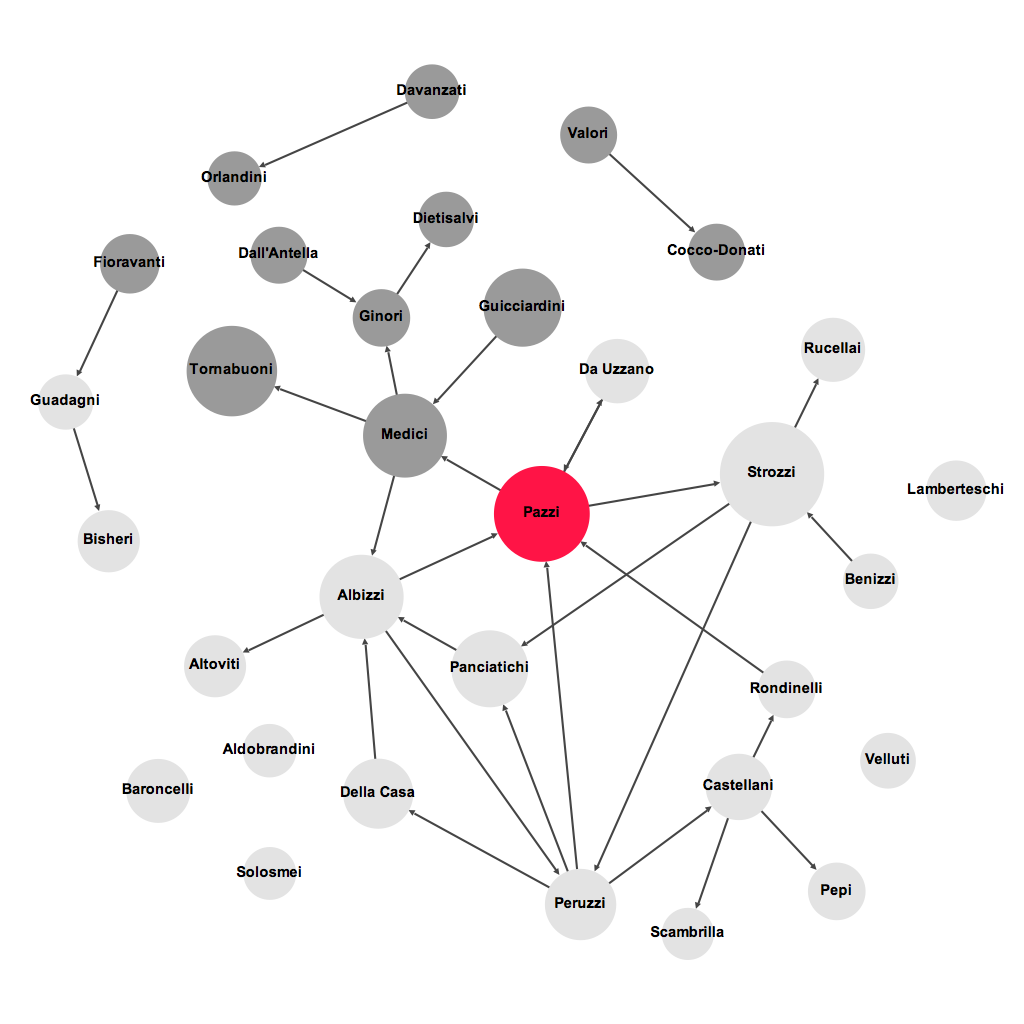
\includegraphics[width=0.9\textwidth]{Images/Florentine-marr.png}
\end{center}
\caption{The Florentine marriage network}
\label{Flocrit}
\end{figure}
Historical analysis by \citet{Roover1946, Roover1963}, \citet{Padgett1993}, and \citet{Goldthwaite2009} attribute the success of the Medician faction during this time to how well organised the faction was relative to the opposing Oligarchic faction. \citet{Padgett1993} suggest that it was common for a member of the oligarchic faction to attempt to overthrow the leadership of its faction and filter information shared with other members. These are indications that there existed a power struggle within the Oligarchic faction. Conversely, in the Medician faction, power is more centralised in the House of Medici itself. It is well accepted that much power was held by the House of Medici, during much of the 15th Century until the Medici were banished from Florence due to inappropriate lending, which lead to war between Italy and France. 

% It may be reasonable to assume that more middlemen and powerful groups exist in the Oligarchic faction than the Medician faction. Indeed, when considering the directed network we identify that more middlemen exist in the Oligarchic faction where power is more distributed. 

Thus, there existed a hierarchical organisation that centred around the House of Medici with little power attributable to other member houses of the faction. This is confirmed in the depicted network: The Medici were positioned at the centre of a star. Although the House of Salviati also has a middleman position, it is clear that the Medici control information flows to the Salviati; indeed, the Medici had the ability of separating the Salviati from the rest of the faction.

The Oligarchic faction were less well-organised. The faction acted more disruptively as power was more distributed throughout the network; this is illustrated by the widespread presence of middlemen in this network. Consequently, it was less centralised with multiple competing houses at various local power centres. In particular, the Houses of Guadagni, Bischeri, Peruzzi, and Castellan all occupy middleman positions, shown in Figure~\ref{Flocrit}. Indeed, up to half of the faction have the potential to control certain channels of communication. Furthermore, the houses of Peruzzi and Strozzi have an incentive to form a coalition to control information flows in the Oligarchic subgraph.

Therefore, there exists more opportunities for power struggles in the Oligarchic faction than the Medician faction. This is representative of the time. It is worth noting that a power struggle occurred within the Medician faction later with respect to the \textit{Pazzi Conspiracy}. And this is conducted through the intervention of the Salviati house, which intermediates the Pazzi and Medici houses in the network.

The preliminary analysis of the elite Florentine marriages moivates us to provide a set of tools to analyse the power of individuals and groups in arbitrary networked environments. The analysis of middlemen in Chapter~\ref{ch:criticalnodes} went some way to providing such an analysis; this chapter generalises the notion of a middleman and generates a normative measure of power with the use of a game theoretic approach to coalition formation.

\paragraph{Chapter outline.}

In this chapter we introduce analytical concepts that try to measure power in an arbitrary directed network. These concepts are supported by two analytical methods, one based on identifying contestation of critical sets and the other founded in a non-cooperative game theoretic analysis that identifies the stable critical structures that emerge in a network. We report that the resulting measures corroborate the historical analysis of the medieval Florentine marriage network presented above.

\subsection{Relationship to the literature}

The work provided here applies the notions of the middleman and critical sets---originally developed in graph theory---to situations in economics and sociology. In social and economic terms, the graph theoretic notion of a critical node is analogous to that of a \emph{middleman}. There exists much work assessing the importance of middlemen in economics. We specifically note seminal work developed by \citet{KalaiMiddlemen1978} which was extended by \citet{JacksonWolinsky1996} and further elaborated upon by \citet{GillesChakrabarti2006} with respect to undirected networks. This literature showed that middleman positions are important in networked intermediation and that such they can extract significant gains from their positions within a cooperative game theoretic framework. Indeed, the insights were analogous to those found by \citet{RubinsteinWolinsky1987}. There also exists much work in sociology regarding middlemen and power. \citet{Emerson1962} illustrates a theory of power relations by assessing the dependence of each player on the other, and thus the number of alternatives that each player has at their disposal for the achievement of a given task. The notions of power--dependence relations were extended to analyse the power of agents in exchange networks by \citet{CookEmersonGillmoreYamagishi1983}. \citet{GouldFernandez1989} note that there can exist multiple types of broker, which acts as a middleman, and provide quantitative measurements for these nodes primarily based on the notion of betweenness centrality. \citet{Gould1989} builds on these early insights, developing a measure for an agents inter--clique brokerage. More recent research has investigated more dynamics of brokerage \citep{Spiro2013}. Despite the vigorous research from both fields into the interlinked notions of middlemen and brokerage, he notion of node cut sets still require intuitive application to scenarios in both sociology and economics. One such article that does this is from~\citet{SimsGilles2014}, who extend the notion of the middleman to that of anti-competitive middlemen. This chapter extends this work by providing an application of cut sets in the form of block formation.

Exploitation and power is closely related to the notion of \emph{competition} in economic systems. Competition has been at the heart of market theory and traditional economics since the formal introduction of Bertrand competition, which claims that if there exists two or more producers for some homogeneous product in a given market then the producers will continually reduce their price levels so that all producers are selling their outputs at the marginal cost of production. The assumption of competitive systems is at the heart of both micro and macroeconomic modelling, however there does not yet exist a broad range of literature regarding competition in networked markets.

\citet{EasleyKleinberg2010} provide a baseline model regarding three classes of players exchanging with each other in a tripartite network subsequently highlighting potential notions of perfect competition and monopolisation. These competitive notions are built from a combination of Bertrand competition and more implicitly from insights of power introduced by \citet{Emerson1962}. \citet{GillesDiamantaris2013} note the importance of middlemen regarding their ability to extract rents from its users that use the platform to interact. The previous chapter provided a formal definition of both strong and weak middlemen in directed networks. In doing so we applied the middleman concept to a network-centric notion of competition, which is effectively a generalisation of Easley and Kleinberg's notion of competition.

\citet{GoyalVega-holes} provides an elaborate example of network formation with surplus--generating economic exchange. The surplus from exchange is split evenly between players that are directly connected and any indirect exchange is split with the set of intermediaries. Players that span structural holes, \'{a} la \citet{Burt1992}, can therefore be highly extractive depending on the players whose exchange they intermediate.

To this point there is a serious deficiency regarding groups of agents collectively attaining extractive positions in networks, comparable to the notion of a \emph{cartel} in economic theory. A procedure proposed by \citet{Aspremont1983} studies the formation of a cartel whereby players announce their willingness to participate in the cartel. A cartel is formed by all players that have announced their willingness to do so. The equilibria of the cartel formation game is characterised by internal and external stability. A cartel is internally stable if no members of the cartel wish to leave, and a cartel is externally stable if no outsider wishes to join the cartel. Drawbacks of the study include that the formation of only a single cartel is considered, and there exists no insights from networks. The integration of a network provides an insightful take on the incentives of cartel formation. Furthermore, we extend the concept to include transfers between players.

We note that the formation of blocks in networks is analogous to the formation of cartels in market economies. However, when applied to networks we find that there can emerge situations where monopolists have an incentive to form a block with other monopolists as well as other powerless players.

\section{Extractive structures in networks}

We introduce the concepts that describe extractive structures in a directed network.

\subsection{Social networks: Basic concepts}

As in Chapter~\ref{ch:criticalnodes} we set out some basic definitions from network theory that help us with our analysis. The concepts and notation are mainly taken from \citet{Jackson2008}. Other standard sources on network theory are \citet{Newman2006book}, \citet{Goyal2007}, \citet{Newman2010} and \citet{Gilles2010}.

We consider a \emph{directed network} as a pair $(N,D)$ where $N=\{1 , 2 , \ldots , n\}$ is a finite set of \emph{nodes}, embodying self-motivated decision-makers, and $D \subset \{(i,j) \mid i,j \in N \mbox{ and } i \neq j\}$ is a set of \emph{arcs}, representing directed links from one node to another.\footnote{We use the notational convention that for two sets $S$ and $T$, we denote by $S \subset T$ that $S$ is included as a subset in $T$ or that $S=T$. Strict inclusion is denoted by $S \subsetneq T$.}

An arc from node $i$ to node $j$ is also denoted by $ij = (i,j)$ which is distinct from $ji = (j,i)$. We remark that our analysis can equally be applied to undirected networks in which all arcs are reciprocated such that $ij \in D$ if and only if $ji \in D$ for all $i,j \in N$.

A \textit{walk} from $i$ to $j$ in a directed network $D$---or an $ij$--\textit{walk}---is an ordered set of nodes $W_{ij} = \{ i_{1}, \ldots ,i_{m} \} \subset N$ with $m \geq 2$, $i_1 =i$, $i_m =j$, and $i_{k}i_{k+1} \in D$ for all $k=1, \ldots ,m-1$. An $ij$--walk $W_{ij}$ from node $i$ to node $j$ in network $D$ is a $ij$--\textbf{path} if there is no $ij$--walk $W'_{ij}$ in $D$ such that $W'_{ij} \subsetneq W_{ij}$. Hence, a path from $i$ to $j$ is a walk from $i$ to $j$ without any loops or cycles.\footnote{This implies that the removal of a node from a $ij$--path will break the connection between $i$ and $j$.}

In many cases there exist multiple paths from $i$ to $j$ in a directed network $D$. Therefore, we denote $W_{ij}^{v}$ as the $v^{th}$ distinct path from $i$ to $j$ in $D$. The class $\mathcal{W}_{ij} (D) = \left\{ W_{ij}^{1}, \ldots ,W_{ij}^{V} \right\}$ consists of all distinct paths from $i$ to $j$ in $D$, where $V = \# \mathcal{W}_{ij}(D)$ is the total number of distinct paths.  If there are no paths from $i$ to $j$, i.e., $V=0$, then $\mathcal{W}_{ij}(D)= \varnothing$. An $ij$--path is a \emph{geodesic path} from $i$ to $j$ in $D$ if it is the path in $\mathcal{W}_{ij} (D)$ with the least number of nodes.

The directed network $D$ is (weakly) \emph{connected} if $\mathcal{W}_{ij}(D) \neq \varnothing$ or $\mathcal{W}_{ji}(D) \neq \varnothing$ or both for all nodes $i,j \in N$. The network $D$ is \emph{strongly connected} if $\mathcal{W}_{ij}(D) \neq \varnothing$ as well as $\mathcal{W}_{ji}(D) \neq \varnothing$ for all nodes $i,j \in N$. Clearly, strongly connected networks are always connected and connected undirected networks are necessarily strongly connected.

If $\mathcal{W}_{ij} (D) \neq \varnothing$, then $j$ is denoted as a \textit{successor} of $i$ in $D$ and $i$ is denoted as a \textit{predecessor} of $j$ in $D$. We let $S_{i}(D)= \{j \in N \mid \mathcal{W}_{ij}(D) \neq \varnothing \}$ as $i$'s \textit{successor set}, where $i \notin S_{i}(D)$. Also, we let $\overline{S}_{i}(D) = S_{i}(D) \cup \{i\}$. Finally, we define $s_{i}(D) = \left\{\, j \in N \,\middle|\, (i,j) \in D \,\right\}$ as the set of \textit{direct successors} of $i$ in $D$. Likewise, $P_{i}(D)=\{j \in N \mid \mathcal{W}_{ji}(D) \neq \varnothing \}$ denotes $i$'s \textit{predecessor set}, where $i \notin P_{i}(D)$ and $\overline{P}_{i}(D) = P_{i}(D) \cup \{i\}$. Here, $p_{i}(D)=\{j \in N \mid (j,i) \in D\}$ is the set of \textit{direct predecessors} of $i$ in $D$.

For a connected network $D$, the node set $N$ can be partitioned into three node classes: Sources; Sinks; and Intermediaries. Node $i \in N$ is a \textbf{source} if $S_{i}(D) \neq \varnothing$ and $P_{i}(D) = \varnothing$; node $i \in N$ is a \textbf{sink} if $S_{i}(D) = \varnothing$ and $P_{i}(D) \neq \varnothing$; and node $i \in N$ in an \textbf{intermediary} if $S_{i}(D) \neq \varnothing$ as well as $P_{i}(D) \neq \varnothing$. In particular, the set of intermediaries in $D$ is introduced as
\begin{equation}
M_D = \{ i \in N \mid S_{i}(D) \neq \varnothing \mbox{ as well as } P_{i}(D) \neq \varnothing \}
\end{equation}
Finally, for any subset of nodes $B \subset N$, we let $D-B$ be defined by
\begin{equation}
D - B = D_{N \setminus B} = \left\{ (j,h) \in D \mid j,h \in N \setminus B \right\} .
\end{equation}
Therefore, $D - B$ is the \emph{restricted} network that results from removing the node set $B$ and all arcs to and from the nodes in $B$.

\subsection{Middlemen and critical sets}

Power in social and economic networks tend to rest on individuals and groups that have an ability to broker relationships and subsequently control information and economic the flows that occur between others in a network.
\begin{definition} \label{Block}
Let $D$ be a directed network on node set $N$ and let $i,j,h \in N$ be distinct nodes.
\begin{abet}

\item A subset of nodes $B \subset N$ is an $ij$--\textbf{critical set} in $D$ if $B \subset \cup \mathcal{W}_{ij}(D) \setminus \{i,j\}$ and $B \cap W_{ij} \neq \varnothing$ for every $ij$--path $W_{ij} \in \mathcal{W}_{ij}(D)$.

\item Node $h$ is an $ij$--\textbf{middleman} in $D$ if the singleton set $\{ h \}$ is a $ij$--critical set in $D$.

\item The collection of critical sets in the network $D$ is given as
\begin{equation}
\mathcal{B}(D) = \left\{ B \subset M_D \mid B \subset N \mbox{ is an $ij$--critical set for some } i,j \in N \, \right\} .
\end{equation}
Also, the set of middlemen in the network $D$ is defined by
\begin{equation}
\mathcal{M}(D) = \left\{ h \in M_D \mid h \mbox{ is an $ij$--middleman for some } i,j \in N \, \right\} .
\end{equation}

\end{abet}
\end{definition}
An $ij$--critical set consists of $ij$--intermediaries that control all flows, communication or intermediation between nodes $i$ and $j$ in network $D$. This implies that these nodes can exercise some form of control in the interaction between the nodes $i$ and $j$. A middleman is a singleton critical set for some pair of nodes. This implies that such a node exercises complete control over all interaction between these two nodes in the network.

Definition~\ref{Block} has equal application to undirected as well as directed networks. A critical set may also contain a middleman or multiple middlemen, but that is not necessary. Also, in an undirected network a critical set is equivalent to a cut set which removal partitions a network into multiple connected components. In particular, a middleman is a cut node in an undirected network.

\begin{figure}[t]
\begin{center}
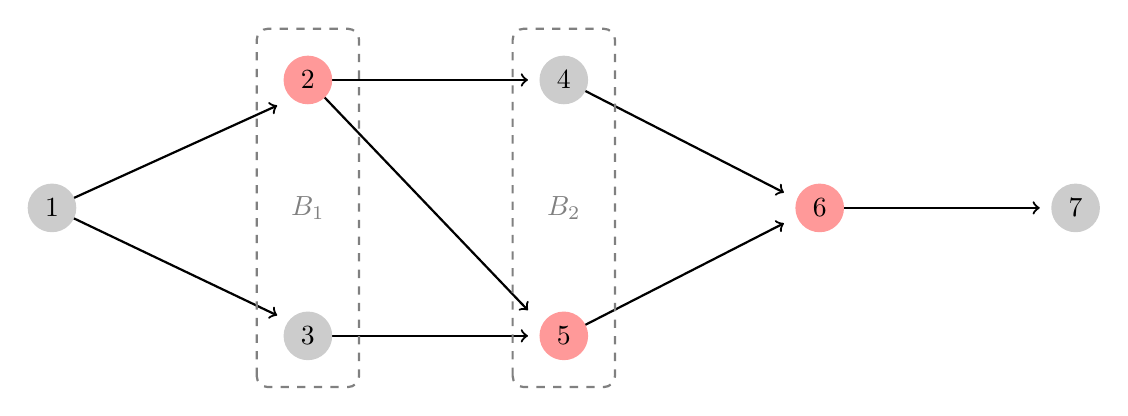
\begin{tikzpicture}[scale=0.65]
\draw[thick, ->] (0,2.5) -- (4.4,4.5);
\draw[thick, ->] (0,2.5) -- (4.4,0.4);
\draw[thick, ->] (5,5) -- (9.3,5);
\draw[thick, ->] (5,0) -- (9.3,0);
\draw[thick, ->] (5,5) -- (9.3,0.5);
\draw[thick, ->] (10,5) -- (14.3,2.8);
\draw[thick, ->] (10,0) -- (14.3,2.2);
\draw[thick, ->] (15,2.5) -- (19.3,2.5);

\draw (0,2.5) node[circle,fill=black!20] {$1$};
\draw (5,5) node[circle,fill=red!40] {$2$};
\draw (5,0) node[circle,fill=black!20] {$3$};
\draw (10,5) node[circle,fill=black!20] {$4$};
\draw (10,0) node[circle,fill=red!40] {$5$};
\draw (15,2.5) node[circle,fill=red!40] {$6$};
\draw (20,2.5) node[circle,fill=black!20] {$7$};

\draw[thick, color=black!50,rounded corners, dashed] (9,-1) rectangle (11,6) ;
\draw[color=black!50] (10,2.5) node {$B_2$} ;

\draw[thick, color=black!50,rounded corners, dashed] (4,-1) rectangle (6,6) ;
\draw[color=black!50] (5,2.5) node {$B_1$} ;

\end{tikzpicture}
\end{center}
\caption{Illustration of critical sets in a network}
\label{Net1}
\end{figure}

\begin{example} \label{ex:Figure1}
To illustrate the concepts introduced here, consider the directed network depicted in Figure 2 on node set $N = \{ 1,2,3,4,5,6,7 \}$. There are three middlemen---or singleton critical sets---in this network, namely node 2 is a $14$--middleman, node 5 is a $36$--middleman and node 6 is a $i7$--middleman for any $i \in \{ 1,2,3,4,5 \}$. These middlemen are represented as the red-shaded nodes in Figure 2.
\\
We also indicate two other critical sets, both supersets of singleton critical sets. The critical set $B_1 = \{ 2,3 \}$ completely controls all connections from node 1 to all other nodes in this network. Similarly, $B_2 = \{ 4,5 \}$ controls the connections of all nodes in $\{ 1,2,3 \}$ with the nodes 6 and 7.
\\
Finally, we mention that connected nodes can form a critical set. Indeed, $B_3 = \{ 2,5 \}$ controls all interaction between nodes in $\{1,3 \}$ and all nodes in $\{ 4,6,7 \}$ and, therefore, is a critical set.
\end{example}
A number of characteristics can be derived for critical sets in a directed network. We state the next properties without proof.
\begin{property} \label{prop:blocks}
Let $D$ be a network on node set $N$ and let $i,j \in N$ with $i \neq j$.
\begin{itemize}
\item[(i)] A node $h \in N$ is a $ij$--middleman in $D$ if and only if
\[
h \in \left[ \, \cap \mathcal{W}_{ij} (D) \, \right] \setminus \{i,j\} .
\]

\item[(ii)] The critical collection $\mathcal{B} (D)$ on network $D$ has properties similar to a \emph{filter} on the set of intermediaries $M_D \subset N$ in the sense that if $B \subset M_D \setminus \{ i,j \}$ is an $ij$--critical set in $D$, then any $B' \subset N$ with $B \subset B' \subset M_D \setminus \{ i,j \}$ is an $ij$--critical set in $D$.

\item[(iii)] Critical sets can be defined in terms of their connectivity role in the network:
\\
If $B \subset N$ is an $ij$--critical set, then it holds that $\mathcal{W}_{ij}(D) \neq \varnothing$ and $\mathcal{W}_{ij}(D - B) = \varnothing$.

\item[(iv)] Let $h \in N$ be an $ij$--middleman and $B \subset N$ such that $h \in B$. Then, $B$ is an $ij$--critical set if and only if $i,j \notin B$.
\end{itemize}
\end{property}
The following theorem addresses the existence of critical sets in a network.
\begin{theorem} \label{thm:noblock}
Let $D$ be a (weakly) connected directed network on $N$. Then $\mathcal{B} (D) \neq \varnothing $ if and only if there exist $i,j \in N$ with $i \neq j$ with a geodesic distance of at least 3, i.e.,
\begin{equation}
\min \left\{ \left. \# W_{ij} \, \right| \, W_{ij} \in \mathcal{W}_{ij} (D) \right\} \geqslant 3 .
\end{equation}
\end{theorem}
\begin{proof}
Let $B \subset N$ be some arbitrary node set. From its definition we deduce that for $B$ to be a critical set between two nodes $i,j \in N$, $i \neq j$, it must be that for all $i,j \notin B \colon B \cap W_{ij}(D) \neq \varnothing$ for every $W_{ij}(D) \in \mathcal{W}_{ij}(D)$.
\\[1ex]
\textbf{Only if:} Suppose to the contrary that $\min \left\{ \# W_{ij} \mid W_{ij} \in \mathcal{W}_{ij}(D) \right\} = 2$. This is the case where $j \in S_{i}(D)$ and, thus, $i \in P_{j}(D)$. Let $W^{\min}_{ij} \in \arg\min \left\{ \# W_{ij} \mid W_{ij} \in \mathcal{W}_{ij}(D) \right\}$ be a geodesic path from $i$ to $j$. Clearly, $\# W^{\min}_{ij}(D) = 2$ implies that $W_{ij}^{\min} \setminus \{i,j\} = \varnothing$. Therefore, $\cap \mathcal{W}_{ij} (D) \setminus \{ i,j \} = \varnothing$ meaning that both there are no nodes to form a critical set for $i$ and $j$.
\\[1ex]
\textbf{If:} Suppose that there exists some $i,j \in N$ where $i \neq j$ such that $\min \left\{ \#W \mid W \in \mathcal{W}_{ij}(D) \right\} \geqslant 3$. Then for every $ij$-path $W \in \mathcal{W}_{ij} (D)$ there exists some node $h_W \in N$ such that $h_W \in W \setminus \{i,j\}$. Define
\begin{equation}
B_{ij} = \left\{ h_W \, \left| \, W \in \mathcal{W}_{ij} (D) \, \right. \right\} \subset N \setminus \{ i,j \} .
\end{equation}
We claim that $B_{ij}$ is a $ij$--critical set in $D$. Indeed, note that for any $ij$--path $W \in \mathcal{W}_{ij} (D)$ it holds that $h_W \in B_{ij} \cap W \neq \varnothing$.
\\[1ex]
This concludes the proof of Theorem \ref{thm:noblock}.
\end{proof}

\bigskip\noindent
We note that this insight identifies an extremely weak requirement for the existence of critical sets in a network. The corollary below indicates this and follows from Theorem~\ref{thm:noblock}.
\begin{corollary}
The following properties hold:
\begin{itemize}
\item[(i)] Let $D$ be any incomplete, non-empty network with at least $3$ nodes that are all connected by a path. Then $\mathcal{B} (D) \neq \varnothing$.

\item[(ii)] $\mathcal{B} (D) = \varnothing$ for both the empty and complete networks.
\end{itemize}
\end{corollary}
\begin{proof}
Following from the proof of Theorem \ref{thm:noblock}, $\mathcal{B}(D) \neq \varnothing$ if and only if there exists a pair $(N,D)$ such that $\# N \geqslant 4$ and at least $4$ nodes are either directly or indirectly connected together such that for some $i,j \in N \colon \min \left\{ \# W_{ij}(D) \mid W_{ij}(D) \in \mathcal{W}_{ij}(D) \right\} \geqslant 3$. Therefore, assertion (i) is shown.
\\[1ex]
Furthermore, Theorem~\ref{thm:noblock} implies that $\mathcal{B} (D) = \varnothing$ if the maximum geodesic path from one node to another in the network is less than $3$, suggesting that there needs to be indirect intermediation between nodes for critical sets to emerge.
\\
In the case of an empty network $D_0 = \varnothing$ on node set $N$, $\mathcal{W}_{ij}(D) = \varnothing$ for all $i,j \in N$. Thus, $\# W_{ij} = 0$ for all $i,j \in N$ and from the above we have that $\mathcal{B} (D) = \varnothing$.
\\
Furthermore, for the complete network $D_N = N \times N$, it holds that $P_{i}(D) = N \setminus \{i\}$ and $S_{i}(D) = N \setminus \{i\}$ for every $i \in N$. Hence, $\min \left\{ \# W_{ij}(D) \mid W_{ij}(D) \in \mathcal{W}_{ij}(D) \right\} = 2$ for all pairs $i,j \in N$. Therefore, $\mathcal{B} (D) = \varnothing$.
\\
This shows assertion (ii).
\end{proof}

\subsection{Network contestability}

In this section we set out to show that the notion of a critical set introduces a topological perspective on competition in networks. Indeed, the nodes that make up these sets are of critical importance to the structure and functioning of a network since their removal leads to both direct and indirect disconnections, propagating a deterioration of the network's functionality. Previously we introduced the notion of network contestability as a descriptor of node-based competition in directed networks. Here we enhance this concept to describe anti-competitive coalition structures in directed networks.

Contestability of a node in a network refers to replacing a node's brokerage function with an alternative arrangement, possibly consisting of multiple nodes. Let $D$ be a network on node set $N$. The \emph{coverage} of a node $i \in N$ is simply defined as $P_{i}(D) \times S_{i}(D)$, i.e., all node pairs that node $i$ serves as an intermediator. A node is now contested if any pair in its coverage can be intermediated by other nodes in the network.

By extension, we can define similar concepts for arbitrary node sets. This is formalised as follows:
\begin{definition}
Let $B \subset N$ be some node set in the directed network $D$. Then the \textbf{coverage} of the node set $B$ in $D$ is given by
\begin{equation} \label{eq:coverageSet}
\Gamma_D (B) =\bigcup_{i \in B} \left\{ \left. \, (h,j) \in ( P_{i} \left( D \right) \setminus B ) \times \left( S_{i} \left( D \right) \setminus B \right) \, \right| \, h \neq j \, \right\}.
\end{equation}
The \textbf{brokerage} of the node set $B$ in $D$ is defined as
\begin{equation}
\Delta_D (B) = \{ (i,j) \in \Gamma_D (B) \mid \mathcal{W}_{ij} (D-B) = \varnothing \}
\end{equation}
\end{definition}
The coverage of a node set $B \subset N$ consists of pairs of nodes that can be intermediated by the nodes in $B$. The brokerage consists of those pairs in the coverage of $B$ that critically depend on the intermediation provided by $B$-members. 

We make a note on the similarity between the coverage of a node set, given by Equation~\ref{eq:coverageSet}, and the coverage noted in Equation~\ref{eq:coverage} in Chapter~\ref{ch:criticalnodes}. Specifically, let $i$ exist in some node set $N$, since $i \notin P_{i}(D)$ and $i \notin S_{i}(D)$, then $i$ cannot exist in it's own coverage. Likewise, given the definition of coverage above, the node set is itself not contained within its coverage. Therefore, let there exist some $B \subset N$ such that $B = \{ i \}$; then $\Gamma_{D}(B) \equiv \Gamma_i (D)$. Indeed this must be true since, by definition, $P_{i}(D) \setminus \{i\} = P_{i}(D)$ and $S_{i}(D) \setminus \{i\} = S_{i}(D)$, therefore if $B = \{i\}$ the equation would simplify to 
\begin{equation}
\Gamma_D (i) = \left\{ \left. \, (h,j) \in P_{i} \left( D \right) \times S_{i} \left( D \right) \, \right| \, h \neq j \, \right\},
\end{equation}
which is equivalent to Equation~\ref{eq:coverage}. As such, the definition of coverage given by Equation~\ref{eq:coverageSet} is a generalisation of coverage given by Equation~\ref{eq:coverage}.

Note the following properties of the coverage and brokerage of node sets.
\begin{property}
Let $D$ be some connected network on node set $N$. Then the following properties hold:
\begin{itemize}
\item[(i)] If $B \subset M_D$ consists of intermediaries only, then $\Gamma_D (B) \neq \varnothing$.

\item[(ii)] $B \in \mathcal{B} (D)$ is a critical set if and only if $\Delta_D (B) \neq \varnothing$.
\end{itemize}
\end{property}
As stated, any critical set $B \in \mathcal{B} (D)$ has the property that at least one pair of nodes in its coverage critically depends on the intermediation of members of that critical set, i.e., $\Delta_D (B) \neq \varnothing$. This property can be formulated by its dual formulation as that the intermediation by its members cannot be contested by nodes outside the critical set. This is set out in the next definition.
\begin{definition} \label{contest}
Let $D$ be a network on node set $N$ and let $B,C \subset N$.
\begin{abet}
\item The node set $C$ \textbf{contests} the node set $B$ if $B \cap C = \varnothing$ and
\begin{equation}
\Gamma_D (B) \subset \bigcup_{j \in C} \left( \, \overline{P}_{j}(D - B) \times \overline{S}_{j}(D - B) \, \right) .
\end{equation}

\item The node set $C$ \textbf{partially contests} the node set $B$ if $B \cap C = \varnothing$ and there is some $j \in C$ such that
\begin{equation}
\Gamma_D (B) \cap \left[ \, \overline{P}_{j}(D - B) \times \overline{S}_{j}(D - B) \, \right] \neq \varnothing.
\end{equation}

\item Node set $B$ is \textbf{uncontested} in $D$ if there is no node set $C \subset N$ such that $C$ contests $B$. Similarly, node set $B$ is \textbf{strongly uncontested} if there is no node set $C \subset N$ such that $C$ partially contests $B$.
\end{abet}
\end{definition}
The distinction between full and partial contestation is that all node pairs in the coverage of a node set $B$ can be intermediated completely by the nodes in $C$ if the nodes in $B$ are removed from the network. Therefore, the intermediation function of the nodes in $B$ can be served fully by nodes in $C$.

Under partial contestation the node set $C$ only can broker the intermediation between a certain number of pairs in $B$'s coverage. The concept of partial contestability allows us to consider the notion of competition in networks in a deeper way. For example, we note that there are networks in which there is \emph{asymmetric contestation} in that node $i$ can contest $j$, but $j$ can only partially contest node $i$.
\begin{example}
Consider the network depicted in Figure~\ref{Net1} and discussed in Example \ref{ex:Figure1}. Clearly, node 2 as a middleman (fully) contests node 3, i.e., node 2 can intermediate all connections between node 1 and the nodes in $\{ 5,6,7 \}$ that are also intermediated by node 3. However, node 3 only partially contests node 2, facilitating the connections between node 1 and nodes 5, 6 and 7, but not that between node 1 and node 4.
\\
We remark that although node 2 is a middleman, it is partially contested by node 3, implying it is not strongly uncontested. However, the interaction between nodes 1 and 4 is always intermediated by node 2; therefore, node 2 is uncontested.
\\
In the example depicted in Figure~\ref{Net1}, middleman 6 is strongly uncontested, since any interaction with node 7 requires intermediation by node 6.
\end{example}
Contestability is a topological representation of a form of competition in a network: It refers to the specific connectivity of nodes in the network as opposed to the actual socio-economic function of these nodes, which is the main focus of traditional ``market competition'' discussed in economic market theory. Therefore, node contestability considers neither the activities of each node, nor the values generated by each node in the network. Instead, we take into consideration the ability of nodes to pass some unchanging output or information through a network.

Critical sets in a network have at least one intermediation that is uncontested by some alternative set of nodes and, therefore, have full control over this intermediation.
\begin{theorem} \label{thm:blockduality}
Let $D$ be some connected network on node set $N$ and let $B \subset N$. The node set $B \in \mathcal{B} (D)$ is a critical set if and only if $B$ is uncontested in $D$.
\end{theorem}
\begin{proof}
Consider a connected network $D$ on $N$. Hence, for every pair $i,j \in N$ it holds that either $\mathcal{W}_{ij} (D) \neq \varnothing$ or $\mathcal{W}_{ji} (D) \neq \varnothing$ or both.
\\[1ex]
\textbf{If:} Let $B \subset N$ be uncontested in $D$. Therefore, $\Gamma_D(B) \neq \varnothing$ and without loss of generality we may assume that $B$ consists of intermediaries only.
\\
Now suppose to the contrary that node set $B$ is not a critical set. Then for \emph{every} pair of nodes $i,j \notin B$ with $i \neq j$, there exists an $ij$-path $\widehat{W}_{ij} \in \mathcal{W}_{ij} (D) \colon B \cap \widehat{W}_{ij} = \varnothing$. We now define
\begin{equation}
C = \bigcup_{i,j \notin B \colon i \neq j} \widehat{W}_{ij} \subset N
\end{equation}
Then $B \cap C = \varnothing$ and any pair $i,j \notin B$ can be intermediated by $C$. Hence,
\[
\Gamma_D (B) \subset \bigcup_{h \in C} \left[ \, \overline{P}_h (D-B) \times \overline{S}_h (D-B) \, \right]
\]
which in turn implies that $C$ contests $B$. This is a contradiction to the hypothesis, proving the assertion.
\\[1ex]
\textbf{Only if:} Suppose that $B \subset N$ is a critical set in $D$. Then there exist some $i,j \notin B$ with $i \neq j$ and $B \cap W \neq \varnothing$ for every path $W \in \mathcal{W}_{ij} (D)$ from $i$ to $j$. This implies that $i$ and $j$ are not connected in $D-B \colon \mathcal{W}_{ij} (D-B) = \varnothing$.
\\
Therefore, it holds that $(i,j) \in \Delta_D (B) \subset \Gamma_D (B)$ as well as that for every node set $C \subset N$ with $B \cap C = \varnothing$ we have
\[
(i,j) \notin \bigcup_{h \in C} \left[ \, \overline{P}_h (D-B) \times \overline{S}_h (D-B) \, \right] .
\]
This shows that $B$ is indeed uncontested.
\end{proof}

\bigskip\noindent
We collect a number of auxiliary properties of critical sets in terms of contestability in the following statement. These properties are quite straightforward and their proofs are therefore omitted.
\begin{property}
Let $D$ be a connected network on node set $N$ with $n \geqslant 3$.
\begin{itemize}
\item[(i)] If $B \subsetneq N \setminus \{ i \}$ for some $i \in N$ is a critical set, then the node set $C = N \setminus \{ i \}$ is contested by $i$, implying that $C$ is not a critical set.

\item[(ii)] Sources have no coverage but have the ability to contest other nodes due to their reach.

\item[(iii)] Let $B \subset N$ be a critical set in the network $D$. Then $B$ must contain all nodes that either contest each other for at least one node pair in its coverage $(i,j) \in \Gamma_D (B)$.
\end{itemize}
\end{property}

\section{Intermediation centrality}

There can exist a large number of critical sets in a network. In fact, the number of critical sets increases proportionally with the number of structural holes \citep{Burt2002} in the network. However, not all of these critical sets in a given network are equally compelling. Here we present a methodology that identifies those critical sets---denoted as \emph{blocks}---that are maximally effective following some plausible measure. In some sense these blocks exercise maximal central control over the intermediation in the network. This allows a game theoretic analysis of selfish control of intermediated connections in a network that lead to these blocks.

The objective function at the foundation of this game theoretic analysis is essential in determining the blocks. This objective function measures the effectiveness of a critical set to control the intermediation it facilitates. Blocks are now exactly the critical sets that in some well-formulated way maximise this objective function.

Formally, an objective function is introduced as an \textbf{intermediation measure}, being a function $\sigma_D \colon \mathcal{B} (D) \to \mathbb{R}$ that assigns to every critical set $B \in \mathcal{B}(D)$ in the network $D$ a number $\sigma_D (B)$ that measures the value of the intermediation provided by $B$'s members to the other nodes in the network. Another interpretation would be that the intermediation measure quantifies the control exercised by members of $B$ over the connections it facilitates in the network $D$.

Examples of intermediation measures are the following measures.
\begin{description}
\item[Filter measure:] As stated in Property \ref{prop:blocks}(ii) the collection of critical sets $\mathcal{B} (D)$ forms a filter on the set of intermediary nodes $M_D$ in the network $D$. The inverse of the number of members of a critical set, therefore, aims to identify the base-elements of that filter.
\\
Formally, the filter measure $\phi_D \colon \mathcal{B}(D) \to \mathbb{R}_+$ is defined as
\begin{equation}
\phi_D (B) = \frac{1}{\# B}
\end{equation}
for every critical set $B \in \mathcal{B} (D)$.

\item[Coverage measure:] A slightly more sophisticated intermediation measure is the one that measures the number of intermediated pairs of nodes. Formally, the \emph{coverage counting measure} is defined as the function $\gamma'_D \colon \mathcal{B} (D) \to \mathbb{N}$ defined by
\begin{equation}
\gamma'_D (B) = \# \Gamma_D (B)
\end{equation}
for every critical set $B \in \mathcal{B} (D)$. The \emph{coverage measure} can be introduced as the function $\gamma_D \colon \mathcal{B} (D) \to \mathbb{Q}$ given by
\begin{equation}
\gamma_D (B) = \frac{\# \Gamma_D (B)}{\# B}
\end{equation}
for every critical set $B \in \mathcal{B} (D)$. It assigns the per-capita number of pairs in the coverage of the critical set in question.

\item[Brokerage measure:] A plausible intermediation measure is founded on the introduced notion of brokerage, which steps up from the coverage measure introduced above. As above, the \emph{brokerage counting measure} is defined as the function $\beta'_D \colon \mathcal{B} (D) \to \mathbb{N}$, which assigns to every critical set $B \in \mathcal{B} (D)$ the size of its brokerage
\begin{equation}
\beta'_D (B) = \# \Delta_D (B) .
\end{equation}
The \emph{brokerage measure} is introduced as the function $\beta_D \colon \mathcal{B}(D) \to \mathbb{Q}$, which assigns to every critical set $B \in \mathcal{B} (D)$
\begin{equation} \label{eq:brokerage}
\beta_D (B) = \frac{\# \Delta_D (B)}{\# B}
\end{equation}
the per-capita number of node pairs that are brokered by $B$ in the network $D$. We remark here that $\beta_D (B) >0$ for all critical sets $B \in \mathcal{B}(D)$.

Clearly, the brokerage measure $\beta_D$ ranks the critical sets in the network $D$ according to the number of node pairs that these critical sets broker, taking account of the size of the critical set considered. Clearly, the brokerage measure introduces a measurement of the desirability of the membership of the critical set if the critical set is viewed as a collaborative coalition of decision makers that try to control the information flows in the network between pairs of connected nodes.

The brokerage measure is used in several applications and examples in the remainder of this paper.

\item[Criticality measure:] The brokerage measure just counts the number of brokered node pairs. A modification of this measure takes into account the effectiveness of this brokerage.
\\
A critical set $B \in \mathcal{B} (D)$ is \emph{non-redundant} if there is no alternative critical set $B' \in \mathcal{B} (D)$ with $B' \subsetneq B$ such that $\Delta_D (B) \subset \Delta_D (B')$. The collection of optimal critical sets is denoted by $\widetilde{\mathcal{B}} (D) \subset \mathcal{B} (D)$.
\\
The \emph{criticality measure} is the intermediation measure $\rho_D \colon \mathcal{B} (D) \to \mathbb{R}$ such that
\begin{equation}
\rho_D (B) = \frac{\max \, \{ \# \Delta_D (B') \mid B' \in \widetilde{\mathcal{B}} (D) \mbox{ and } B' \subset B \, \}}{\# B} .
\end{equation}
The criticality measure assigns to every critical set the per-capita brokerage of its most effective or optimal subset in terms of brokerage. It refers to the widest brokerage that is offered by its members in the network.

\end{description}
The introduction of the general class of control measures allows for the study of alternative ways to quantify the control exercised by a node set in a network.

\subsection{Block structures}

If an intermediation measure quantifies the effectiveness of the brokerage provided by the members of a critical set in a network, then the critical sets that maximise this intermediation measure can be identified as the most effective brokerage node sets. We denote these critical sets as \emph{blocks}.
\begin{definition} \label{def:block}
Let $D$ be a network on the node set $N$ such that $\mathcal{B} (D) \neq \varnothing$ and let $\sigma \colon \mathcal{B} (D) \to \mathbb{R}$ be an intermediation measure on $D$.
\\
We define a $\sigma$-\textbf{block structure} as a finite collection $\mathcal{P} (\sigma ) = \left\{ \, B^1, \ldots ,B^K \, \right\} \subset \mathcal{B} (D)$ of critical sets in the network $D$, which is constructed through the following algorithm:
\begin{itemize}
\item[(i)] Select
\[
B^1 \in \arg\max \left\{ \, \sigma (B) \, \middle| \, B \in \mathcal{B} (D) \, \right\}
\]
and define
\[
\mathcal{A}^1 = \left\{ \, B \in \mathcal{B} (D) \, \middle| \, B \cap B^1 = \varnothing \, \right\} .
\]

\item[(ii)] Let $\{ B^1 , \ldots ,B^m \}$ be selected and let $\mathcal{A}^m$ be as constructed. Then select
\begin{equation}
B^{m+1} \in \arg\max \left\{ \, \sigma (B) \, \middle| \, B \in \mathcal{A}^m \, \right\}
\end{equation}
and construct
\begin{equation}
\mathcal{A}^{m+1} = \left\{ \, B \in \mathcal{A}^m \, \middle| \, B \cap \left( \cup^{m+1}_{k=1} B^k \right) = \varnothing \, \right\} .
\end{equation}

\item Continue with \emph{(ii)} until $\mathcal{A}^K = \varnothing$.
\end{itemize}
The collection of all $\sigma$-structures in $D$ as defined above is denoted by  $\mathbf{P} ( \sigma )$.
\\
Every critical set that is part of a $\sigma$-block structure $B \in \cup \mathbf{P} (\sigma ) \subset \mathcal{B} (D)$ is called a $\sigma$-\textbf{block}. The collection of all $\sigma$-blocks is denoted by $\widehat{\mathcal{B}} (\sigma ) \subset \mathcal{B} (D)$.
\end{definition}
A $\sigma$-block structure is a collection of critical sets $B \in \mathcal{B} (D)$ with a maximal intermediation measure $\sigma (B)$ in the network $D$. The notion of a block now captures those critical sets that are members of at least one $\sigma$-block structure. These are the most preferred critical sets in the sense that nodes in these critical sets exercise maximal control over the connections that they mediate.

The properties of the network $D$ and selected control measure $\sigma$ determine how many blocks there emerge. The next theorem states the exact condition under which there emerges a minimal number of blocks, namely a collection of critical sets that make up a unique maximal control pattern. The following properties are again stated without proof.
\begin{property}
Let $D$ be a network on node set $N$ such that $\mathcal{B} (D) \neq \varnothing$ and let $\sigma \colon 2^N \to \mathbb{R}$ be some intermediation measure on $D$. Then the following properties hold.
\begin{itemize}
\item[(i)] If $\sigma$ is discerning in the sense that $\sigma (B) \neq \sigma_D (B')$ for all distinct critical sets $B,B' \in \mathcal{B} (D)$ with $B \neq B'$, then there exists a unique $\sigma$-block structure on $D$.

\item[(ii)] The $\phi$-blocks based on the filter measure $\phi \colon \mathcal{B} (D) \to \mathbb{R}_+$ form the base elements of the filter system of critical sets $\mathcal{B} (D)$ on the set of intermediaries $M_D$ in $D$. Hence, the $\phi$-blocks are exactly the set-theoretically minimal critical sets in the network $D$; this includes the set of middlemen $\mathcal{M} (D)$.
\end{itemize}
\end{property}
We conclude the discussion of block structures and blocks with a simple example that exemplifies the different block structures that are supported by different intermediation measures in the same network.

\begin{figure}[h]
\begin{center}
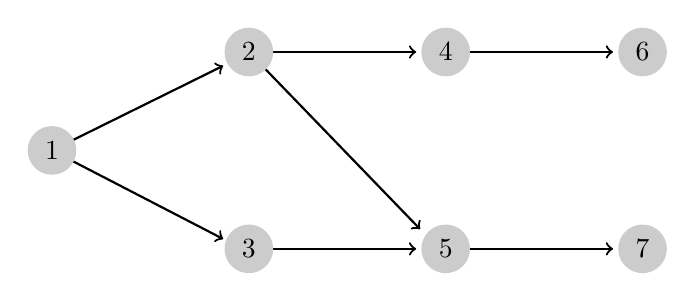
\begin{tikzpicture}[scale=0.5]
\draw[thick, ->] (0,2.5) -- (4.35,4.65);
\draw[thick, ->] (0,2.5) -- (4.35,0.25);
\draw[thick, ->] (5,5) -- (9.35,0.5) ;
\draw[thick, ->] (5,5) -- (9.25,5);
\draw[thick, ->] (5,0) -- (9.25,0);
\draw[thick, ->] (10,5) -- (14.25,5);
\draw[thick, ->] (10,0) -- (14.25,0);

\draw (0,2.5) node[circle,fill=black!20] {$1$};
\draw (5,5) node[circle,fill=black!20] {$2$};
\draw (5,0) node[circle,fill=black!20] {$3$};
\draw (10,5) node[circle,fill=black!20] {$4$};
\draw (10,0) node[circle,fill=black!20] {$5$};
\draw (15,5) node[circle,fill=black!20] {$6$};
\draw (15,0) node[circle,fill=black!20] {$7$};

\end{tikzpicture}
\end{center}
\caption{The network $D_1$ considered in Example \ref{ex:comparison}}
\label{Fig2}
\end{figure}

\begin{example} \label{ex:comparison}
Consider the network $D_1$ depicted in Figure~\ref{Fig2} on the node set $N = \{ 1,2,3,4,5,6,7 \}$. We remark that node $3$ is the only contested node among the four intermediary nodes in this network. We consider a subclass of critical sets in the network $D_1$: The middlemen $\{ 2 \}$, $\{ 4 \}$ and $\{ 5 \}$ and the multi-node critical sets $B_1 = \{ 2,3 \}$, $B_2 = \{ 2,5 \}$, $B_3 = \{ 3,4 \}$ and $B_4 = \{ 4,5 \}$. Other critical sets are supersets and unions of these listed (relevant) critical sets.
\\
We now consider all block structures in the network $D_1$ that are generated for the coverage measure $\gamma$ and the brokerage measure $\beta$.\footnote{It is remarked here that there is no difference between the criticality measure $\rho$ and the brokerage measure $\beta$ in the network $D$ used this example, i.e., $\rho_D (B) = \beta_D (B)$ for all critical sets $B \in \mathcal{B} (D)$.}
\begin{itemize}
\item With regard to the coverage measure $\gamma$ on $D_1$ we remark that $\gamma (2) =4$, $\gamma (4) = 2$ and $\gamma (5) =3$. Furthermore, $\gamma (B_1) = \gamma (B_2) = \gamma (B_3) = \tfrac{4}{2}=2$ and $\gamma (B_4) = \tfrac{5}{2}=2 \tfrac{1}{2}$.
\\
There emerge two $\gamma$-block structures in the network $D_1$ given by
\begin{align*}
\mathcal{P}_1 (\gamma ) & = \{ \, 2, 5 , B_3 \, \} \\
\mathcal{P}_2 (\gamma ) & = \{ \, 2, 4 , 5 \, \}
\end{align*}

\item The brokerage measure $\beta$ applied to the network $D_1$ results in the assignment $\beta (2) = \beta (4) =2$, $\beta (5) =3$, $\beta (B_1) = \beta (B_2) = \tfrac{4}{2} =2$, $\beta (B_3) = \tfrac{2}{2}=1$ and $\beta (B_4) = \tfrac{5}{2} = 2 \tfrac{1}{2}$. Given these brokerage values we deduce that there emerge two $\beta$-block structures:
\begin{align*}
\mathcal{P}_1 (\beta ) & = \{ \, 2, 4 , 5 \, \} \\
\mathcal{P}_2 (\beta ) & = \{ \, B_1 , 4 , 5 \, \}
\end{align*}
\end{itemize}
These computations show that different intermediation measures might lead to the identification of the same block structure ($\mathcal{P}_2 (\gamma ) = \mathcal{P}_1 (\beta )$) or different block structures in the network. In particular, $B_1$ is a $\beta$-block, but not a $\gamma$-block, while $B_3$ is a $\gamma$-block, but not a $\beta$-block.
\end{example}

\subsection{A game-theoretic approach to intermediation centrality}

An intermediation measure assigns to every critical set the perceived power of control it exercises in the network. Therefore, if the nodes are controlled or occupied by intelligent decision makers, such an intermediation measure can act as an objective function in a ``block formation process''. Indeed, these decision makers seek membership of critical sets that exercise maximal control over connections between other nodes in the network.

There is direct relationship between such a block formation process and the creation of a multi-sided platform in the sense of \citet{HagiuWright2015}. The resulting block can be interpreted as the provision of a platform provided by its members through which node pairs interact.

The formation of a block requires consent from all members. As such the block formation game described is considered to be an augmented version of \citeauthor{Myerson1991}'s network formation game \cite[see][page 448]{Myerson1991}. We argue that this is the most natural format to describe the process of block formation: If there exists no consent between players then the block becomes dysfunctional and its exploitive properties are nullified. Some characteristics from \citeauthor{Myerson1991}'s game remain, however by implementing the game on an existing network some new characteristics are observed. Specifically we note that individual beliefs and expectations can be formed from knowledge of the network's topology which leads to more convincing self-confirming equilibria \citep{GillesSarangi2010}.

\subsubsection{Block formation games}

Let $D$ be some network on node set $N$ and let $\sigma_D \colon \mathcal{B} (D) \to \mathbb{R}$ be some intermediation measure that assigns every critical set a commonly accepted measurement of its control power in the network $D$. Also, introduce $c \geqslant 0$ be a cost parameter. Formally, the corresponding \textbf{block formation game} is now introduced as a strategic form game $G (D, \sigma_D ,c ) = (N,S, \pi )$ where $N$ is the set of nodes, interpreted as the set of decision makers or ``players''; $S = (S_1, \ldots ,S_n )$ is an assignment of a strategy set to every player $i \in N = \{ 1, \ldots ,n \}$; and $\pi \colon \prod_{i \in N} S_i \to \mathbb{R}^N$ is a game-theoretic payoff function that assigns to every strategy tuple $s = (s_1, \ldots ,s_n)$ a payoff vector $\pi (s) = (\pi_1 (s), \ldots ,\pi_n (s))$ such that the following holds:
\begin{itemize}
\item For every player $i \in N$ the strategy set is defined as
\begin{equation}
S_i = \mathcal{B}_i (D) \cup \{ i_0 \} ,
\end{equation}
where $\mathcal{B}_i (D) = \{ B \in \mathcal{B} (D) \mid i \in B \}$ is the set of critical sets of which $i$ is a member. The status quo strategy $i_0 \in S_i$ means that node $i$ chooses to be no member of any critical set in the network $D$.
\\
If $i \in N$ is a middleman, then clearly $\{ i \} \in \mathcal{B}_i (D)$ and the strategy $\{ i \}$ refers to the choice of $i$ to exercise control over her intermediated node pairs.

\item For every player $i \in N$ the payoff function $\pi_i \colon \prod_{i \in N} S_i \to \mathbb{R}$ is given by
\begin{equation}
\pi_i (s) = \sum_{B \in \mathcal{B}_i (D)} \kappa (s,B) \cdot \sigma_D (B) - \left( \, \# s_i -1 \, \right) c
\end{equation}
where $c \geqslant 0$ is a block formation cost parameter and $\kappa \colon \left( \prod_{i \in N} S_i \right) \times \mathcal{B} (D) \to \{ 0,1 \}$ is an indicator function with
\begin{equation}
\kappa (s,B) = \left\{
\begin{array}{ll}
1 & \mbox{if } s_j = B \mbox{ for all } j \in B \\
0 & \mbox{otherwise}
\end{array}
\right.
\end{equation}
We remark that $\kappa (s,B)$ indicates whether a critical set is actually formed through the consent of its members or not. Hence, $\kappa (s,B)=1$ signifies that the critical set $B$ is formed by consent from all its member nodes. Since $s_i$ is unique, it is clear that the payoff $\pi_i (s)$ only emanates from the chosen critical set of which node $i$ wants to become a member.
\end{itemize}
The given formulation of a block formation game represents that nodes as decision makers aim to optimise the returns on the control-exercise activities they participate in. We assume that such blocking is exclusive and nodes can only participate in a single active critical set.

The game-theoretic payoff function is based on that all players use the same assessment of the power of control potentially exercised by a critical set, expressed by the intermediation measure $\sigma_D$. All nodes are assumed to pay for the coordination of their blocking activities and to pay a communication cost of $c \geqslant 0$ to each other member of the selected block. Critical sets only emerge when all of the constituting nodes consent and agree to participate.

Finally, we emphasise that it is costless to exercise one's middleman position or to remain inactive completely. Indeed, in the case, $s_i = \{ i \}$ the resulting payoff is simply given by $\pi_i (s) =\sigma_D ( \{ i \} )$ irrespective of the strategies selected by the other players in the block formation game. Together with the above, this implies that every strategy tuple in a block formation game generates a coalition structure on the set of nodes given by the following:
\begin{definition}
Let $G (D, \sigma_D ,c ) = (N,S, \pi )$ be the block formation game on the network $D$ based on the intermediation measure $\sigma_D \colon \mathcal{B} (D) \to \mathbb{R}$ and communication cost parameter $c \geqslant 0$.
\\
The \textbf{coalition structure} corresponding to a strategy tuple $s \in \prod_{i \in N} S_i$ is the collection $\mathcal{C} (s) = \{ B^1, \ldots ,B^M \} \subset 2^N$ of mutually disjoint subsets of $N$ defined for every $m \in \{ 1, \ldots ,M \}$ by the rule that for every node $i \in B^m$ it holds that either $B^m \in \mathcal{B}_i (D)$---in case that $\kappa (s, B^m)=1$ and $s_i = B^m$---or $B^m = \{ i \}$---in case that $\kappa (s,B^m) =0$.
\\
For every node $i \in N$ we denote by $C_i (s) \subset N$ the set $B \in \mathcal{C} (s)$ such that $i \in B$.
\end{definition}
The coalition structure corresponding to some strategy tuple consists of the subsets of nodes that either form a critical set and all of its members agree on forming it, or form a singleton if there is no agreement on the formation of a critical set.

We now can derive the following properties of a block formation game.
\begin{theorem}
Let $G (D, \sigma_D ,c ) = (N,S, \pi )$ be some block formation game on the network $D$ based on the intermediation measure $\sigma_D \colon \mathcal{B} (D) \to \mathbb{R}$ and the communication cost parameter $c \geqslant 0$. Then the following properties hold.
\begin{itemize}
\item[(i)] The block formation game $G (D, \sigma_D ,c ) = (N,S, \pi )$ is a potential game in the sense of \citet{MondererShapley1996} for the potential function $\mathbf{P} \colon \prod_{i \in N} S_i \to \mathbb{R}$ given by
\[
\mathbf{P} (s) = \sum_{B \in \mathcal{B} (D)} \kappa (s,B) \cdot \sigma_D (B) - \sum_{i \in N} \# C_i (s) \, c .
\]

\item[(ii)] The block formation game $G (D, \sigma_D ,c) = (N,S, \pi )$ admits at least one Nash equilibrium.

\item[(iii)] In particular, the trivial strategy $s^0 \in \prod_{i \in N} S_i$ given by $s^0_i = i_0$ is a Nash equilibrium in the block formation game $G (D, \sigma_D ,c) = (N,S, \pi )$ such that $\mathcal{C} (s^0) = \{ \, \{ i \} \mid i \in N \}$.

\item A critical set $B \in \mathcal{B} (D)$ emerges through some Nash equilibrium in $G (D, \sigma_D ,c) = (N,S, \pi )$ if and only if there is no node $i \in B \colon \sigma_D (\{ i \}) > \sigma_D (B) - (\# B -1)c$.
\end{itemize}
\end{theorem}
\begin{proof}
Assertion (i) follows immediately from checking the potential function properties of $\mathbf{P}$ in relationship to the game theoretic payoff function $\pi$.
\\[1ex]
Assertion (ii) is implied by assertion (iii), which rests on the fact that if all players select the status quo strategy, then no non-middleman critical set can be formed by modification of a single player's strategy. Thus, $s^0_i \equiv i_0 \in S_i$ is a best response to $s^0_{-i}$ irrespective of the values generated by $\sigma_D$ and the cost level $c \geqslant 0$.
\\[1ex]
It remains to show assertion (iv).
\\
The formation of a critical set $B \in \mathcal{B} (D) \setminus \mathcal{M} (D)$ requires consent from all of its members. Hence, if there is some $i \in B \colon \sigma_D (\{ i \}) > \sigma_D (B) - (\# B -1)c$, then $\pi_{i}(s) > \pi_{i}(s')$ where $s_{i} = \{ i \}$, $s'_{i} = B \in \mathcal{B}_i (D)$, and $s_{-i} = s'_{-i}$. This implies that $B$ cannot be supported through a Nash equilibrium in the block formation game.
\\
If there is no $j \in B \colon \sigma_D (\{ j \}) > \sigma_D (B) - (\# B -1)c$, then player $i$ will have no incentive to exploit her own position unless there is some $j \in B$ such that $s_{j} \neq B$ and $c > 0$. In either case $B$ will not form in a Nash equilibrium.
\\
This implies assertion (iv) and completes the proof of the theorem.
\end{proof}

\subsection{Stability in the formation of block structures}

Consider the block formation game $G (D, \sigma_D ,c) = (N,S, \pi )$ on network $D$ based on intermediation measure $\sigma_D$ and communication cost parameter $c \geqslant 0$. Then a strategy tuple $s^* \in \prod_{i \in N} S_i$ is a \emph{strong Nash equilibrium} \citep{Aumann1959} if for every non-empty coalition of players or nodes $B \subset N$ with $B \neq \varnothing$ and every $s_B \in \prod_{j \in B} S_j$ it holds that if $\pi_j (s_B, s^*_{N \setminus B}) > \pi_j (s^*)$ for some player $j \in B$, then there is some player $h \in B \colon \pi_h (s_B, s^*_{N \setminus B}) < \pi_h (s^*)$.

Our main result is that $\sigma$-structures exactly correspond to the strong Nash equilibria of the zero-cost block formation game. Hence, all coalitions generated in a strong Nash equilibrium of a zero-cost block formation game are indeed $\sigma$-blocks.
\begin{theorem} \label{thm:SNE-block}
Let $D$ be a connected network on $N$ with $\mathcal{B} (D) \neq \varnothing$ and let $\sigma_D \colon \mathcal{B} (D) \to \mathbb{R}$ be an intermediation measure on the network $D$. Assume that communication is costless $(c=0)$. Then the following hold:
\begin{itemize}
\item[(i)] Every $\sigma_D$-block structure as introduced in Definition \ref{def:block} can be supported through a strong Nash equilibrium in the corresponding zero-cost block formation game $G (D, \sigma_D ,0)$.

\item[(ii)] For every strong Nash equilibrium $s^*$ in the zero-cost block formation game $G (D, \sigma_D ,0)$, the generated structure $\mathcal{C} (s^*) \cap \mathcal{B} (D)$ is a $\sigma_D$-block structure on $D$.
\end{itemize}
\end{theorem}
\begin{proof}
Let $\sigma_D \colon \mathcal{B} (D) \to \mathbb{R}$ be an intermediation measure on $D$ and let $G (D, \sigma_D ,0) = (N,S, \pi )$ be the corresponding zero-cost block formation game.
\\[1ex]
\textbf{Proof of (i):}
Let $\mathcal{P} (\sigma_D) = \left\{ \, B^1, \ldots ,B^K \, \right\} \subset \mathcal{B} (D)$ be a $\sigma$-block structure as in Definition \ref{def:block}.
\\
In the zero-cost block formation game $G (D, \sigma_D ,0) = (N,S, \pi )$ define a strategy tuple $\hat{s} \in \prod_{i \in N} S_i$ that is given as follows:
\begin{itemize}
\item For any $k \in \{ 1, \ldots ,K \}$ and any player $i \in B^k$ select $\hat{s}_i = B^k \in \mathcal{B}_i (D)$, and

\item for any player $j \in N \setminus \left( \cup_{k=1}^K B^k \right)$ select $\hat{s}_j = j_0$.
\end{itemize}
We now claim that $\hat{s}$ is a strong Nash equilibrium of $G (D, \sigma_D ,0)$ and that $\mathcal{P} (\sigma_D) \subset \mathcal{C} (\hat{s})$. Suppose to the contrary that there exists some $B \subset N$ and some strategy tuple $s_B \in \prod_{i \in B} S_i$ with $\pi_i (s_B, \hat{s}_{N \setminus B}) > \pi_i (\hat{s})$ for all players $i \in B$. Without loss of generality, due to the payoff function, we may assume that $B \in \mathcal{B} (D)$ and that $s_B (i) = B$ for every $i \in B$. Therefore, for every $k \in \{ 1, \ldots ,K \}$ and every $i \in B \cap B^k$ it holds that $\pi_i (s_B , \hat{s}_{N \setminus B}) = \sigma_D (B) > \pi_i (\hat{s}) = \sigma_D (B^k)$.
\\
But this contradicts the definition of $\mathcal{P} (\sigma_D)$ as a $\sigma_D$-block structure. Indeed, the critical set $B$ identified above should have emerged from the algorithmic selection process described in Definition \ref{def:block} and, thus, $B^{k'} =B$ for some $k' \in \{ 1, \ldots ,K \}$.
\\[1ex]
\textbf{Proof of (ii):}
Let $s^* \in \prod_{i \in N} S_i$ be a strong Nash equilibrium in $G (D, \sigma_D ,0)$. Let the corresponding structure be denoted by $\mathcal{C} (s^*) \cap \mathcal{B} (D) = \{ \widehat{B}^1, \ldots , \widehat{B}^M \}$.
\\
Suppose to the contrary that $\mathcal{C} (s^*) \cap \mathcal{B} (D)$ is not a $\sigma_D$-block structure on $D$. Then for some $m \in \{ 1, \ldots ,M \}$ there exists some $\sigma_D$-block $B \in \mathcal{B} (D)$ such that $\sigma_D (B) > \sigma_D (\widehat{B}^m)$ and $B \cap \widehat{B}^m \neq \varnothing$. But then all $j \in B$ could improve upon $s^*$ by coordinating on the formation of $B$. This contradicts the hypothesis that $s^*$ is a strong Nash equilibrium in $G (D, \sigma_D ,0)$.
\end{proof}

\subsection{Brokerage centrality analysis}

As an interesting case of the framework developed here is that of the brokerage intermediation measure $\beta$ defined in equation (\ref{eq:brokerage}). This intermediation measure results in some interesting properties and can be applied to study data from historic socio-economic networks.
\begin{theorem} \label{thm:beta-block}
Let $\beta_D \colon \mathcal{B} (D) \to \mathbb{R}_+$ be the brokerage measure on the network $D$. Then the following properties hold:
\begin{itemize}
\item[(i)] Every $\beta_D$-block $B \in \cup \mathbf{P} (\beta_D)$ is non-redundant in the sense that $B \in \widetilde{\mathcal{B}} (D)$, i.e., there is no strictly smaller critical set $B' \subsetneq B$ such that $\Delta_D (B) \subset \Delta_D (B')$.

\item[(ii)] Let $B \in \mathcal{B} (D)$ be a critical set such that it contains a strongly uncontested node $i \in B$. If $\beta_D (\{ i \}) \neq \beta_D (B) - (\# B-1) c$ for some $c \geqslant 0$, then $B$ is not supported to form in any strong Nash equilibrium in the block formation game $G (D, \beta_D ,c)$.
\end{itemize}
\end{theorem}
\begin{proof}
Let $D$ be some network on node set $N$. \\[1ex]
\textbf{Proof of assertion (i):}
Let $B \subset N$ be a redundant $\beta_D$-block in the sense that there exists a strict subset $B' \subsetneq B$ with $\Delta_D (B) \subset \Delta_D (B')$. Since $\# B' < \# B$ and $\# \Delta_D (B) \leqslant \# \Delta_D (B')$ it follows by definition that $\beta_D (B') > \beta_D (B)$. But this contradicts that $B$ is assumed to satisfy the definition of a $\beta_D$-block given in Definition \ref{def:block}.
\\[1ex]
\textbf{Proof of assertion (ii):} Note that the node $i \in B$ is a middleman, since it is strongly uncontested. Hence, $\{ i \} \in \mathcal{B} (D)$.
\\
First consider the case that $\beta_D (\{ i \}) = \# \Delta_D (i) > \beta_D (B) - (\# B-1)c$. Then, obviously, the middleman $i$ rather forms a status quo singleton cialition $\{ i \}$ by herself than being member of $B$. Therefore, $B$ is never a best response for $i$, excluding $B$ from forming in a Nash equilibrium at costs level $c$.
\\
Next consider the case that $\beta_D (\{ i \}) = \# \Delta_D (i) < \beta_D (B) - (\# B-1)c$. Let $B-i = B \setminus \{ i\}$. Since $i$ is strongly uncontested, it follows that $\Delta_D (B) = \Delta_D (B-i) \cup \Delta_D (i)$ and $\Delta_D (B-i) \cap \Delta_D (i) = \varnothing$. Thus, $\# \Delta_D (B) = \# \Delta_D (B-i) + \# \Delta_D (i)$. Therefore,
\begin{align*}
\beta_D (B-i) - (\# (B-i) -1)c & = \frac{\# \Delta_D (B-i)}{\# B-1} - (\# B-2) c = \\[1ex]
 & = \frac{\# \Delta_D (B) - \# \Delta_D (i)}{\# B-1} - (\# B-2) c > \\[1ex]
 & > \frac{\# \Delta_D (B) - \left[ \, \tfrac{\# \Delta_D (B)}{\# B} - (\# B-1)c \, \right]}{\# B-1} - (\# B-2) c = \\[1ex]
 & = \frac{\# \Delta_D (B)}{\# B} - (\# B-3)c > \frac{\# \Delta_D (B)}{\# B} - (\# B-1)c = \\[1ex]
 & = \beta_D (B) - (\# B-1)c
\end{align*}
Hence, in the block formation game $G (D, \beta_d ,c)$, the coalition $B-i$ provides a strictly higher payoff than the coalition $B$ for its member nodes. Therefore, $B$ can never be resulting in a strong Nash equilibrium in the block formation game. This shows the assertion.
\end{proof}

\subsubsection{An illustrative example}

Consider network $D$ on node set $N=\{1,2,3,4,5,6,7\}$ originally shown in Figure~\ref{Net1}. Players $2$, $5$, and $6$ are middlemen and there exists $66$ distinct critical sets. However, only $3$ of these critical sets are non-redundant in the sense of Theorem \ref{thm:beta-block}.

\begin{figure}[h]
\begin{center}
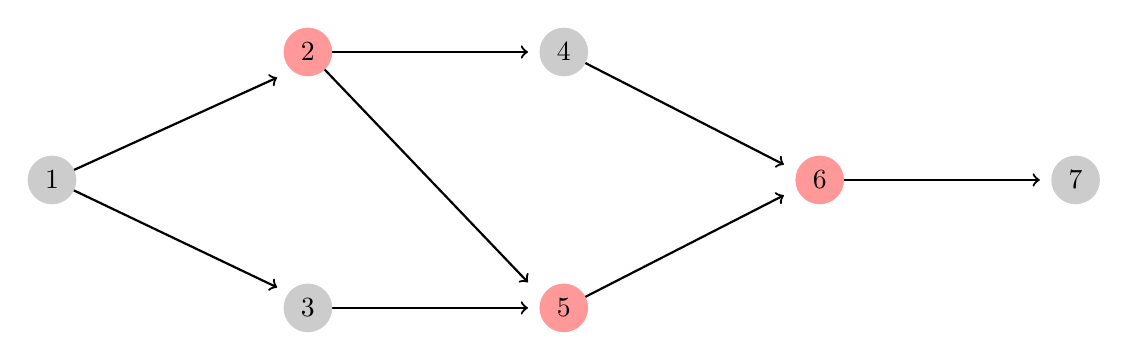
\begin{tikzpicture}[scale=0.65]

\draw[thick, ->] (0,2.5) -- (4.4,4.5);
\draw[thick, ->] (0,2.5) -- (4.4,0.4);
\draw[thick, ->] (5,5) -- (9.3,5);
\draw[thick, ->] (5,0) -- (9.3,0);
\draw[thick, ->] (5,5) -- (9.3,0.5);
\draw[thick, ->] (10,5) -- (14.3,2.8);
\draw[thick, ->] (10,0) -- (14.3,2.2);
\draw[thick, ->] (15,2.5) -- (19.3,2.5);

\draw (0,2.5) node[circle,fill=black!20] {$1$};
\draw (5,5) node[circle,fill=red!40] {$2$};
\draw (5,0) node[circle,fill=black!20] {$3$};
\draw (10,5) node[circle,fill=black!20] {$4$};
\draw (10,0) node[circle,fill=red!40] {$5$};
\draw (15,2.5) node[circle,fill=red!40] {$6$};
\draw (20,2.5) node[circle,fill=black!20] {$7$};

\end{tikzpicture}
\end{center}
\caption{Middlemen in network $D_1$}
\end{figure}

We now consider the block formation game $G (D, \beta_D ,c)$ based on the brokerage measure $\beta_D$ and communication cost parameter $c \geqslant 0$. For different cost levels there emerge different stable block structures in the network and different critical sets emerge in the resulting strong Nash equilibria.\footnote{We recall that only for zero-cost communication, the strong Nash equilibria in the block formation game results into $\beta_D$-blocks in this network.} We explore these patterns below.
\begin{description}
\item[For $\mathbf{0 \leqslant c < 1}$:]
There exists a unique strong Nash equilibrium in $G (D, \beta_D ,c)$ in which there emerges the partitioning $\langle \{ 1 \} , \{2,3\} , \{4,5\} , \{ 6 \} , \{ 7 \} \rangle$. Player $6$ will never have any incentive to form a larger block since it is strongly uncontested.
\\
There exist multiple Nash equilibria (NE) in $G (D, \beta_D ,c)$. Without going through all different combinations of these equilibria we can instead note that the only critical sets that can form in a Nash equilibrium are the following: $B = \{2,3\}$, $B' = \{4,5\}$, $B'' = \{2,5\}$ for $c \leqslant 0.5$; and $B''' = \{2,3,4\}$ for $c=0$. Block $B''$ is notable as it consists of middlemen only. Block $B'''$ is notable as it is non-redundant and still stable in the resulting Nash equilibria.

\item[For $\mathbf{c = 1}$:]
There exist four strong Nash equilibria:
\begin{itemize}
\item[(1)] The partitioning $\langle \{ 1 \} , \{2,3\} , \{4,5\} , \{ 6 \} , \{ 7 \} \rangle$;
\item[(2)] An SNE resulting in the partitioning $\langle \{ 1 \} , \{2,3\} , \{4 \}, \{5\} , \{ 6 \} , \{ 7 \} \rangle$;
\item[(3)] An SNE resulting in the partitioning $\langle \{ 1 \} , \{2\} , \{3\} , \{4,5\} , \{ 6 \} , \{ 7 \} \rangle$; and
\item[(4)] An SNE that results in the trivial non-cooperation equilibrium in which all nodes act solitary given by $\langle \{ 1 \} , \{ 2\} ,\{ 3\} , \{ 4 \} , \{ 5 \} , \{ 6 \} , \{ 7 \} \rangle$.
\end{itemize}
In this case the set of Nash equilibria in $G (D, \beta_D ,c)$ are equal to the set of SNE. Indeed, only two blocks are stable in NE: $B=\{2,3\}$ and $B'=\{4,5\}$. Obviously the situation in which all agents exploit their own network position is also a NE.

\item[For $\mathbf{c > 1}$:]
There exists a unique strong Nash equilibrium in $G (D, \beta_D ,c)$ where every node $i \in N$ acts solitary. Indeed, if $c > 1$ then players $2$ and $5$ strictly prefer to exploit their own middleman positions as opposed to participating in some block. Under this situation the only agents that earn a payoff above zero are the middlemen. Again, the unique Nash equilibrium is equal to the unique SNE such that all agents exploit their own position only.
\end{description}
The illustration and discussion highlights a number of points made through the discussion. First, that non-redundant critical sets can emerge in a Nash equilibrium, but not in a strong Nash equilibrium. Second, that the emerging blocks can contain solely middlemen, or non-middlemen, or a combination of both.

\section{Some applications}

Next we apply the framework developed in the previous sections to two cases, namely to the medieval Florentine marriage network---depicting the information flows between houses in the Florentine elite in the 15th century---and to the 9/11 terrorist network as it developed between 1999 and the attack in September 2001.

In order to apply the developed notions we introduce a method to derive a node centrality measure from any intermediation measure introduced in Section 3. We use intermediation measures to measure and quantify the control critical sets of nodes have in the prevailing network. We can allocate this measure to the individual nodes in these critical sets.

For that purpose we recall that $\mathcal{B} (D)$ denotes the collection of all critical sets in network $D$ and that $\mathcal{B}_i (D)$ denotes the collection of critical sets that node $i \in N$ is a member of. Furthermore, $\widetilde{\mathcal{B}} (D) \subset \mathcal{B} (D)$ is the collection of non-redundant critical sets.

Now, an intermediation measure $\sigma_D \colon \mathcal{B} (D) \to \mathbb{R}$ \emph{induces} a centrality measure $\overline{\sigma} (D) \colon N \to \mathbb{R}$ given by
\begin{equation}
\overline{\sigma}_i (D) = \frac{1}{S (\sigma_D)} \sum_{B \in \mathcal{B}_i (D)} \sigma_D (B) \quad \mbox{where } S(\sigma_D) = \sum_{B \in \mathcal{B} (D)} \sigma_D (B) .
\end{equation}
This naturally introduces the coverage and brokerage centrality measures $\overline{\gamma}$ and $\overline{\beta}$, respectively, derive from the coverage intermediation measure $\gamma_D$ and the brokerage intermediation measure $\beta_D$, respectively.

Furthermore, the intermediation measure $\sigma_D$ induces a collection of $\sigma_D$-blocks denoted by $\widehat{\mathcal{B}} (\sigma_D) \subset \mathcal{B} (D)$. This naturally leads to a brokerage centrality measure that is restricted to these blocks:
\begin{equation}
\widehat{\rho}_i (D) = \sum_{B \in \widehat{\mathcal{B}}_i (D)} \rho_D (B) =  \sum_{B \in \widehat{\mathcal{B}}_i (D)} \frac{\# \Delta_D (B)}{\# B} .
\end{equation}
Here, as before, $\widehat{\mathcal{B}}_i (D)$ denotes the collection of $\sigma_D$-blocks that $i \in N$ is a member of.

For completeness, we introduce a normalisation of the centrality measure $\widehat{\rho}_i (D)$ above, founded on the collection of non-redundant critical sets $\widetilde{\mathcal{B}} (D) \subset \mathcal{B} (D)$. Thus, we define
\begin{equation}
\overline{\rho}_i (D) = \frac{1}{\widetilde{S} (\sigma_D)} \sum_{B \in \widetilde{\mathcal{B}}_i (D)} \rho_D (B) \quad \mbox{where } \widetilde{S} (\sigma_D) = \sum_{B \in \widetilde{\mathcal{B}} (D)} \rho_D (B) .
\end{equation}
We apply these centrality measures to analyse different directed networks. Before doing so we provide an overview as to the circumstances in which to use the aforementioned centrality measures. After this, we show through application to the Florentine elite network that the centrality brokerage measure based on non-redundant critical sets is actually redundant. First, however, we note that the centrality measures developed involve NP-hard problems. The number of non-redundant blocks need to be calculated, for example, this can require assessing all other potential node sets in the network; a problem that has a time complexity class of $O(2^n)$.

\subsection{Applying centrality measures}

Through the game theoretical development of block formation we provided three normalised centrality measures defined on an arbitrary set of nodes. These set centrality measures referred to coverage centrality ($\overline{\gamma}$), brokerage centrality ($\overline{\beta}$) and criticality ($\overline{\rho}$). All of these centrality measures are similar in that they are explicitly derived from the set of walks that the nodes are positioned on; however, they measure different aspects of nodes within the network. We discuss the differences between the measures and the application of these measures on network data sets. Specific outcomes of the overview are that as we move from coverage to brokerage to criticality we get measures that specifically highlight more powerful nodes in controlling flows within the network, and that criticality is the only measure that considers a potentially dynamic network of intelligent actors.

First, coverage centrality measures all potential flows that contain the specific node or node set in the network. We note that each node has a potential to combine with other nodes to increase their coverage. Due to this, the coverage of a node will always be greater than zero for non-trivial networks.

Second, brokerage centrality is a measurement that surmises all of a given nodes opportunities to broker information and trade within the network. Thus, regardless of whether a node is a middleman, a non-middleman intermediary, a source, or a sink they can potentially have an individual brokerage centrality of above zero. This is because nodes can form blocks within the network; this measure analyses the blocks regardless of whether they were to rationally form under any condition. Each nodes ability to broker flows within a networked system therefore depends both on their individual position, and the position of other nodes within the networked environment.

Finally, criticality is only defined on the non-redundant blocks that can exist within some Strong Nash equilibrium of the block formation game. As a consequence, fewer nodes within the network will have a criticality above zero. Sources, sinks and isolated singletons, for example, will have a criticality of exactly zero. This filtering of important nodes provides a more precise indication of the most important sets of nodes. This is particularly prevalent in situations where, given the structure of the network, it is strategic for nodes to coordinate their activities. Indeed, this is the only measurement of centrality that makes sense when considering a dynamic network consisting of individual actors with some degree of rationality.

Each centrality measure developed should be considered in order to find different aspects of a node and different types of network. Each measure should be used under different situations. For example, when considering a situation where strategic activity is possible, such as collusion, the measurement of criticality would highlight aspects of a nodes importance that may not be highlighted by other measures. Likewise, if we are considering a rigid network within which information flows between nodes, then the measure of brokerage would provide the most insightful results.

\subsection{The Florentine elite network: A further analysis}

The coverage, brokerage, and criticality of all elite Florentine families are given in Table~\ref{table:florentineElite}. There are a total of $132,474$ critical sets that can potentially form in the directed marriage network. However, most of these include sources and sinks. Indeed, there result a total of $1,020$ critical sets consisting of intermediaries only. Only $36$ of these critical sets are non-redundant.

From the table we find that the Medici family have the largest relative brokerage centrality $\overline{\beta}$. This is specifically because of their substantial middleman position in the network and the number of critical sets that they are members of. The total number of which is $512$. The Pazzi, Albizzi, and Strozzi houses have brokerage scores close to that of the Medici's. These were obviously also important families during this time and close rivals to the Medici in both politics and finance. Due to their closeness they participate in as many critical sets as the Medici. However, we note that the Peruzzi and Rondinelli families are only seen as modestly important with respect to the brokerage measure, despite the families forming the unique non-singleton block in the network. We note that all sources, sinks and singletons of the directed marriage network attain a criticality score of $0$ and will, as such, never have membership of a non-redundant block.

Surprisingly, both the coverage centrality $\overline{\gamma}$ and criticality $\overline{\rho}$ measures diminish the importance of the Medici relative to other Houses in the network. The family is ranked as joint third highest according to the criticality measure and joint top with five other Houses according to the coverage centrality measure $\overline{\gamma}$. Indeed, despite differences in brokerage, criticality, and other centrality measures, many families have identical coverage centrality scores; including the Medici and other top familes. This is due to the presence of families that are members of the same strongly connected component or are members of strongly connected components of the same size, for example, singletons.

The relative reduction in the House of Medici's criticality can be explained specifically due to their prominence as middlemen. They only participate in $4$ non-redundant critical sets specifically as a consequence of their powerful middleman position in the network. Indeed, any critical set that the Medici are a member of, becomes redundant because the Medici could achieve a superior payoff by operating independently. Thus, as a consequence of this middleman power, for any critical set that the House of Medici is a member of, there always exists a subset that contains the Medici family and has a superior brokerage than the initial critical set. These two centrality measures give a higher value to houses that have a less substantial middleman positions and are in many more non-redundant critical sets, such as the Rondinelli, Peruzzi and Castellani families. Indeed, it is a general phenomenon that with the criticality measure the centrality score of intermediary agents tend to converge; this is because non-middleman intermediaries now have an ability to form extractive structures that have a greater potential to be non-redundant.

\begin{table}[H]
\begin{center}
\begin{tabular}{llccc}
\toprule
House 	& Faction 	& $\overline{\gamma}_{i}$	& $\overline{\beta}_{i}$	& $\overline{\rho}_{i}$	\\
\midrule
Albizzi(**)			& Oligarch 			& 0.175			& 0.252 		& 0.428	\\
Aldobrandini		& Oligarch 			& 0.106 		& 0.099 		& 0.000	\\
Altoviti			& Oligarch 			& 0.099 		& 0.094 		& 0.000	\\
Baroncelli			& Oligarch 			& 0.106 		& 0.099 		& 0.000	\\
Benizzi				& Oligarch 			& 0.095 		& 0.089 		& 0.000	\\
Bisheri 			& Oligarch 			& 0.103 		& 0.099 		& 0.000	\\
Castellani(**)		& Oligarch 			& 0.175 		& 0.161 		& 0.358	\\
Cocco-Donati  		& Medician 			& 0.106 		& 0.099 		& 0.000	\\
Da Uzzano  			& Oligarch 			& 0.103 		& 0.085 		& 0.000	\\
Dall'Antella 		& Medician 			& 0.106 		& 0.099 		& 0.000	\\
Davanzati   		& Medician 			& 0.106 		& 0.099 		& 0.000	\\
Della Casa  		& Oligarch 			& 0.103 		& 0.084 		& 0.066	\\
Dietisalvi 			& Medician 			& 0.096 		& 0.089 		& 0.000	\\
Fioravanti  		& Medician 			& 0.103 		& 0.099 		& 0.000	\\
Ginori(**)  		& Medician 			& 0.125 		& 0.123 		& 0.292	\\
Guadagni(**)  		& Oligarch 			& 0.127 		& 0.102 		& 0.099	\\
Guicciardini 		& Medician 			& 0.096 		& 0.087 		& 0.000	\\
Lamberteschi		& Oligarch 			& 0.106 		& 0.099 		& 0.000	\\
Medici(**)   		& Medician 			& 0.175 		& 0.327 		& 0.374	\\
Orlandini  			& Medician 			& 0.106 		& 0.099 		& 0.000	\\
Panciatichi 		& Oligarch 			& 0.103 		& 0.090 		& 0.066	\\
Pazzi(**)   		& Mixed 			& 0.175 		& 0.311 		& 0.511	\\
Pepi        		& Oligarch 			& 0.099 		& 0.091 		& 0.000	\\
Peruzzi(*)  		& Oligarch 			& 0.175 		& 0.222 		& 0.395	\\
Rondinelli(*) 		& Oligarch 			& 0.175 		& 0.115 		& 0.272	\\
Rucellai     		& Oligarch 			& 0.098 		& 0.092 		& 0.000	\\
Scambrilla 			& Oligarch 			& 0.099 		& 0.091 		& 0.000	\\
Solosmei    		& Oligarch 			& 0.106 		& 0.099 		& 0.000	\\
Strozzi(**) 		& Oligarch 			& 0.174 		& 0.170 		& 0.374	\\
Tornabuoni   		& Medician 			& 0.099 		& 0.092 		& 0.000	\\
Valori     			& Medician 			& 0.106 		& 0.099 		& 0.000	\\
Velluti     		& Oligarch 			& 0.106 		& 0.099 		& 0.000	\\
\bottomrule
\end{tabular}
\end{center}
\caption{Centrality measures for the Florentine elite network in Figure~\ref{Flocrit}}
\label{table:florentineElite}
\end{table}

Finally, despite the large number of blocks in the network there exists a brokerage block structure whereby all families exploit their own position apart from the Panciatichi and the Della Casa who form the unique non-trivial $\beta$-block. Both families are members of the same faction and there exists no direct relationship between the families. It should be noted, though, that the families formed a relationship during the prolonged fall of the Medici. As the legacy of the \textit{Pazzi Conspiracy} became ingrained into the Florentine elite and the Medici began to lose their stronghold in Florence, families between factions became connected through marital ties. One such inter-faction marriage was between the house of Albizzi and the house of Tornabuoni as Giovanna degli Albizzi married to Lorenzo Tornabuoni. The Albizzi family were at the centre of the Oligarchic faction and the main family to rival the Medici. Note how the middleman power of the Medici is substantially reduced given the marriage between the Albizzi and Tornabuoni, which impacts the Medici's dominence. As the Medici's power declined the members of the Albizzi family began to befriend members of the Medici family and took some of the roles of the Medici when they were banished from Florence. Indeed, Luca Albizzi became the \textit{Gonfalonier of Justice} and later remained a key ally of the Medici.

We conclude that the coverage centrality measure $\overline{\gamma}$ as well as the criticality measure $\overline{\rho}$ are less descriptive than the brokerage centrality measure $\overline{\beta}$ for the analysis of the power of the Medici family. The following analysis of the 9/11 terrorist network is therefore restricted to those two measures.

\subsection{The 9/11 terrorist networks}

The notions of blocks and criticality are applied to the terrorist cell involved in the organisation and attack of the World Trade Centre and the Pentagon on September 11, 2001 (hereby addressed as ``9/11''). We consider the terrorist cell as an evolving social network, highlighting four time periods that show how the terrorists became connected to one another during the lead-up to the attack. The network is constructed to allow us to investigate the role of middlemen and blocks in the organisation of the terrorist attack.

Whereas the Florentine marriage network investigated information flows in a largely non-cooperative environment, the network of 9/11 terrorists is an example of information flows in a co-operative environment. As a consequence the notion of blocks can be perceived in a different manner: in this case blocks highlight sets of individuals that are required for the stability of the terrorist operation. The removal of blocks would deteriorate the cooperation and information flow between a large number of terrorists in the network. The blocks that are formed in the Strong Nash equilibrium therefore represent sets of nodes that are important for network dismantlement and destruction; which is a core topic in much of network science \citep{Carley2002, Carley2006, KovacsBarabasi2015, MoroneMaske2015}. Indeed, the algorithm for defining blocks could equally be used for network dismantlement and costly optimised vaccination strategies.

As before, the brokerage of a node represents the number of relationships that the node brokers through all of the critical sets that they can participate in. The criticality of a node represents the number of relationships that the node brokers in all non-redundant critical sets that the node can participate in. This criticality measure therefore provides a better indication of the number of relationships that the individual node will broker. Here, we assess the brokerage and criticality of all individual terrorists in order to see the terrorists most instrumental to the coordination and information flow throughout the terrorist network. Unlike other assessments of the terrorist network \citep{Krebs2002, Farley2003, Lindelauf2013, Flores2014} we investigate the evolution of the network over time. Specifically, we assess the criticality of the individuals across four time periods during the run-up to the terrorist attack, these time periods are: January 1999, December 2000, May 2001, and August 2001. The social structure of the 9/11 terrorists across these time periods are seen in chronologically in Figures \ref{Terrorist-Jan99}, \ref{Terrorist-Dec00}, \ref{Terrorist-May01} and \ref{Terrorist-Aug01}.

\paragraph{Data.}

Data was gathered from a number of sources. The largest source of data regarding the development of the terrorist cell network over time was from \emph{The History Commons}\footnote{The complete 9/11 timeline can be found on The History Commons website at \href{http://www.historycommons.org}{http://www.historycommons.org}.} and \citet{Thompson2004}. However, information was also collected from The 9/11 Commission Report, from a technical report on the \emph{Joint Inquiry into Intelligence Community Activities Before and After the Terrorist Attacks of September 11}, from a technical report provided by the CIA on \emph{11 September: The Plot and the Plotters} and from a working paper by \citet{MassonWilkins2013}. The information gathered from these sources allowed us to reconstruct the social network of the terrorist cell.

We first provide some summary statistics on the evolution of the network structure over the time periods, then provide some discussion on the criticality of individual terrorists in the network.

\subsubsection*{Network structure}

The summary statistics of all networks are given in Table \ref{TerroristSS}. We analyse the social relationships between 32 distinct terrorists, all of which are connected to the 9/11 attacks. The initial network contains 27 terrorists, this increases to 31 terrorists, then 32 terrorists by August 2001. By May 2001 the 4 strongly connected components in January 1999 reduce down to a single strongly connected component by August 2001. The effective diameter of the network\footnote{The effective diameter of a network is the 90th percentile distance between any two nodes. See \citet{Leskovec2005a} for more details on this measure.} remains close to 4 for all time periods. And the average path length shortens from a peak of 2.510 in December 2000 to 1.991 in August 2001.

Over time the average number of connections per node in the social network increases, indicating a greater integration of the social network. The measures of density and modularity can look misleading without the context of the number of nodes and the number of network components and communities. As the network evolves the original nodes become more connected to each other and broad bridges between communities exist. The maximal $k$-core is 7 for all networks due to the existence of the dense community of eight terrorists\footnote{Containing the individuals Mamoun Darkazanli, Mohammad Atta, Mohammed Haydar Zammar, Marwan Al-Shehhi, Said Bahaji, Ziad Jarrah, Mounir El Motassadeq, and Zakariya Essabar.}, all of which met previously as members of a terrorist cell operating in Hamburg. This indicates the existence of a network of terrorists prior to the plans and implementation of the 9/11 attack, and also indicates the inability for a subset of this group to broker information across all other members.

\begin{table}[h]
\begin{center}
\begin{tabular}{lcccc}
\toprule
& \multicolumn{4}{c}{Terrorist network} \\[1ex]
Statistic			& Jan 1999 	& Dec 2000 	& May 2001 	& August 2001 	\\
\midrule
Size ($n$)         & 27      & 31       & 31         & 32          \\
\# of links        & 62      & 82       & 99         & 127         \\
\# of components   & 4       & 2        & 1          & 1           \\
\# of communities  & 6       & 5        & 3          & 3           \\
Avg. degree        & 4.593   & 5.290    & 6.392      & 8.000       \\
Avg. path length   & 2.332   & 2.510    & 2.283      & 1.991       \\
Effective diameter & 4       & 5        & 4          & 4           \\
Density            & 0.183   & 0.171    & 0.214      & 0.253       \\
Modularity         & 0.463   & 0.472    & 0.430      & 0.362       \\
Critical sets      & 589,709 & 886,772  & 1,109,989  & 1,181,994   \\
$\sigma$-blocks    & 27      & 168      & 217        & 68          \\
\bottomrule
\end{tabular}
\end{center}
\caption{Summary statistics describing the evolution of the 9/11 terrorist network}
\label{TerroristSS}
\end{table}

The modularity of the network decreases as more links are made between nodes and the operation becomes more cohesive. Moreover, the number of non-redundant blocks falls substantially given the increased cohesion of the terrorist network in August 2001 prior to the September attacks, even though the number of critical sets containing all intermediaries increases.

\subsubsection*{Brokerage and criticality}

The brokerage and criticality results for all 9/11 terrorists are provided in Table~\ref{allterrorists} for reference. A shorter table of the most critical terrorists across all time periods can be seen in Table~\ref{criticalterrorists}.

The criticality of each individual node, denoted by $\overline{\rho}(i)$, corresponds well with the brokerage of the node, denoted by $\overline{\beta}(i)$, such that the overall correlation coefficient between the average brokerage and average criticality of the set of terrorists is 0.668. A number of terrorists have persistently high brokerage and criticality across all time periods, indicating that their requirement for the functioning and coordination of the terrorist cell. These are Hani Hanjour, Hamza Alghamdi, Khalid Sheikh Mohanned (KSM), and Nawaf Al-Hazmi. It is satisfying to note that these actors were seen as key implementers by \emph{The Office of the Director of National Intelligence}, and other studies noted above. The social structure and the tools that we developed in order to analyse the criticality of individual nodes in networks are able to highlight these key coordinators.

\begin{table}[t]
\begin{center}
\begin{tabular}{lrr}
\toprule
 & \multicolumn{2}{c}{Average across all years} \\[1ex]
Name 			   & $\overline{\beta}_{i}$ 	& $\overline{\rho}_{i}$	\\
\midrule
Hani Hanjour        & 0.553   & 0.304   \\
Nawaf Al-Hazmi      & 0.370   & 0.372   \\
Hamza Alghamdi      & 0.310   & 0.336   \\
Waleed Al-Shehri    & 0.306   & 0.253   \\
KSM                 & 0.276   & 0.249   \\
Ahmed Alghamdi      & 0.254   & 0.202   \\
Khalid Al-Mihdhar   & 0.230   & 0.172   \\
Ahmed Alnami        & 0.221   & 0.155   \\
Mustafa Al-Hisawi   & 0.218   & 0.160   \\
Mohamed Atta        & 0.211   & 0.302   \\
\bottomrule
\end{tabular}
\end{center}
\caption{Top 10 ranked terrorists in terms of average $\overline{\beta}_{i}$ across all time periods}
\label{criticalterrorists}
\end{table}

Consider the graphs regarding the evolution of the terrorist network over the four time periods assessed. The coloured nodes distinguish high brokerage blocks that form as a result of the SNE of the game described in the chapter: nodes of a given solid colour represents the nodes that participate in a given block together. We can see that as the network densifies the size of the blocks that appear in the SNE become larger. The largest in January 1999 is 3 and the largest in May and August 2001 is 5; this suggests that as the network grows information transmission between any two nodes becomes more robust and that dismantling the network becomes more costly. However, individual brokers still exist; specifically, Hani Hanjour maintains his position as a middleman from December 2000 to August 2001, being the pilot and coordinator of the American Airlines Flight 77 to crash into the Pentagon.

It is often found that members of a block in the SNE are not connected to each other directly, but connected through a single intermediary. Consider the example of Nawaf Al-Hazmi and Waleed Al-Shehri who are always a member of a significant SNE block, but are never connected to one another directly. This may have been considered as a strategic move: if terrorists were captured or removed then it is more likely for their neighbours to be removed also due to tracking and interrogation; if members of significant blocks are closely connected to each other then the block as a whole is prone to removal thus fracturing communication throughout the network.

\begin{subappendices}

\section{Visualising 9/11 terrorist networks}

The network diagrams regarding the evolution of the 9/11 terrorist network is given below. Significant SNE blocks are depicted as coloured nodes. A single block has a single colour attached.

\begin{figure}[h]
\begin{center}
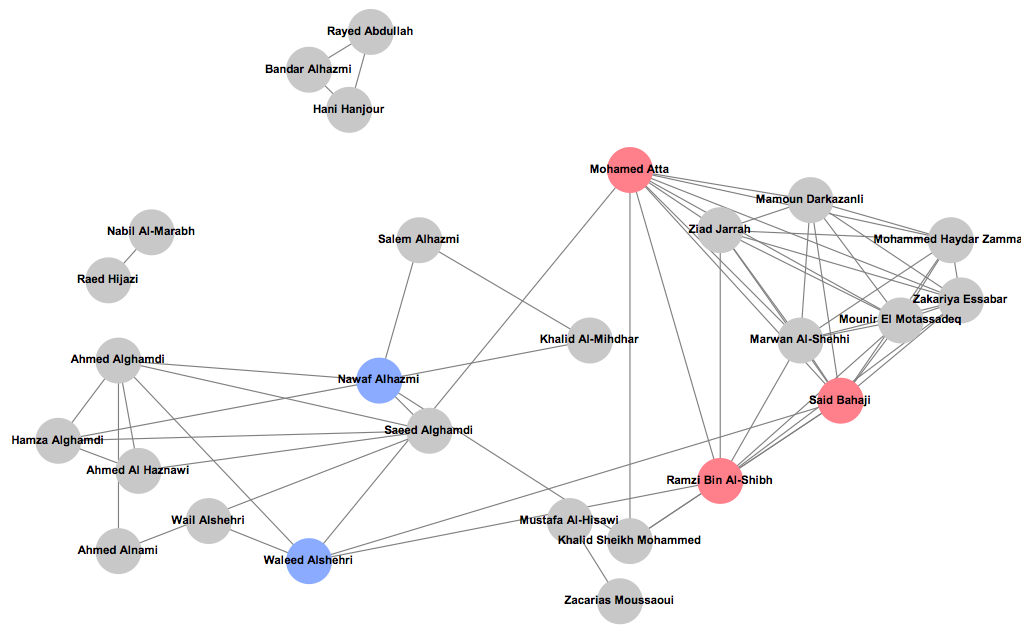
\includegraphics[scale=0.4]{Images/T1999-01.png}
\end{center}
\caption{The 9/11 terrorist network in January 1999}
\label{Terrorist-Jan99}
\end{figure}

\begin{figure}[h]
\begin{center}
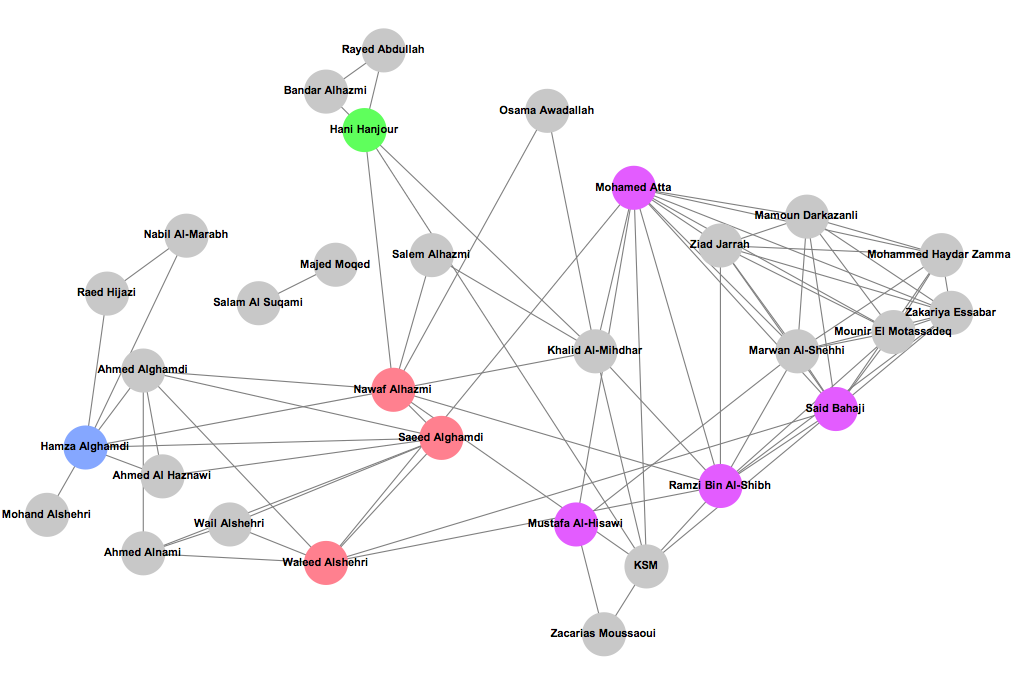
\includegraphics[scale=0.4]{Images/T2000-12.png}
\end{center}
\caption{The 9/11 terrorist network in December 2000}
\label{Terrorist-Dec00}
\end{figure}

\begin{figure}[h]
\begin{center}
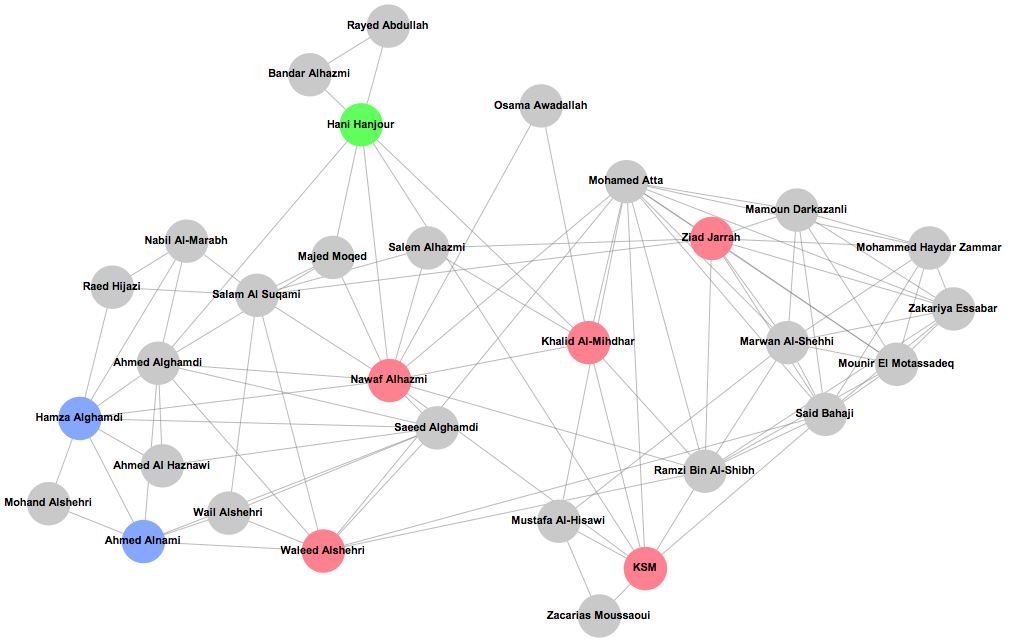
\includegraphics[scale=0.4]{Images/T2001-05.png}
\end{center}
\caption{The 9/11 terrorist network in May 2001}
\label{Terrorist-May01}
\end{figure}

\begin{figure}[h]
\begin{center}
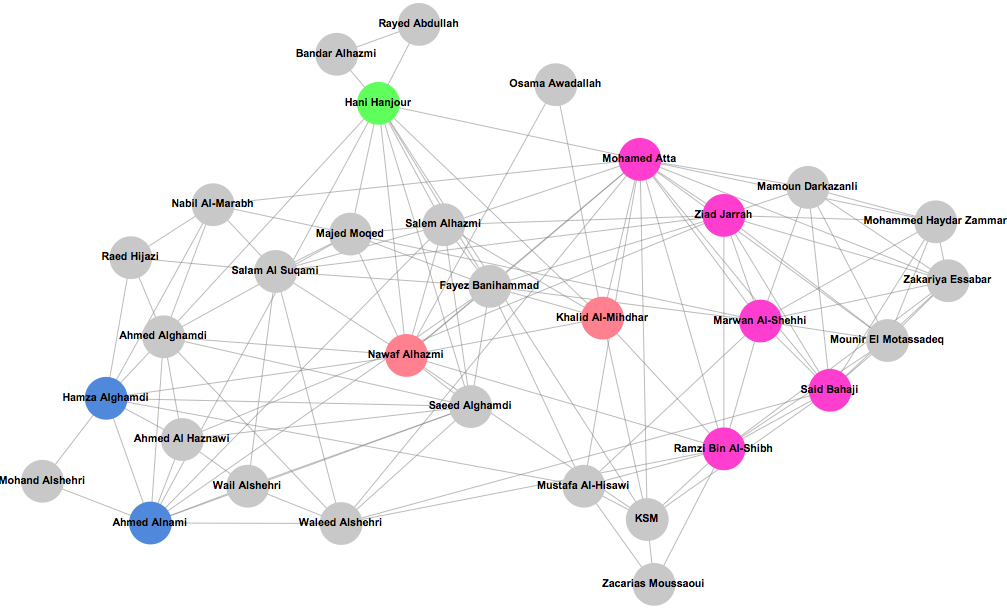
\includegraphics[scale=0.4]{Images/T2001-08.png}
\end{center}
\caption{The 9/11 terrorist network in August 2001}
\label{Terrorist-Aug01}
\end{figure}

\newpage

\begin{sidewaystable}[t]
\begin{center}
\begin{tabular}{l cc cccccccc}
\toprule
 & \multicolumn{2}{c}{Jan 1999} & \multicolumn{2}{c}{Dec 2000} & \multicolumn{2}{c}{May 2001} & \multicolumn{2}{c}{Aug 2001} & \multicolumn{2}{c}{Average} \\[1ex]
\midrule
Name  & $\overline{\beta}_{i}$ & $\overline{\rho}_{i}$ & $\overline{\beta}_{i}$ & $\overline{\rho}_{i}$ & $\overline{\beta}_{i}$  & $\overline{\rho}_{i}$ & $\overline{\beta}_{i}$ & $\overline{\rho}_{i}$ & $\overline{\beta}_{i}$ & $\overline{\rho}_{i}$ \\
\midrule
Ahmed Al-Haznawi      	& 0.195	  & 0.024   & 0.198   & 0.028   & 0.181   & 0.000   & 0.183   & 0.058   & 0.189   & 0.028   \\
Ahmed Alghamdi        	& 0.388   & 0.031   & 0.324   & 0.033   & 0.221   & 0.508   & 0.185   & 0.237   & 0.254   & 0.202   \\
Ahmed Alnami          	& 0.191   & 0.016   & 0.202   & 0.012   & 0.241   & 0.264   & 0.250   & 0.327   & 0.221   & 0.155   \\
Bandar Alhazmi        	& 0.219   & 0.000   & 0.070   & 0.000   & 0.118   & 0.000   & 0.109   & 0.000   & 0.155   & 0.000   \\
Hamza Alghamdi        	& 0.200   & 0.000   & 0.510   & 0.388   & 0.278   & 0.445   & 0.252   & 0.510   & 0.310   & 0.336   \\
Hani Hanjour          	& 0.219   & 0.000   & 0.392   & 0.259   & 0.751   & 0.456   & 0.851   & 0.500   & 0.553   & 0.304   \\
Khalid Al-Mihdhar     	& 0.172   & 0.000   & 0.254   & 0.051   & 0.244   & 0.406   & 0.250   & 0.230   & 0.230   & 0.172   \\
Mamoun Darkazanli     	& 0.202   & 0.006   & 0.201   & 0.031   & 0.182   & 0.000   & 0.183   & 0.000   & 0.192   & 0.009   \\
Marwan Al-Shehhi      	& 0.202   & 0.021   & 0.213   & 0.040   & 0.201   & 0.142   & 0.184   & 0.384   & 0.200   & 0.147   \\
Mohamed Atta          	& 0.226   & 0.283   & 0.232   & 0.112   & 0.203   & 0.312   & 0.184   & 0.500   & 0.211   & 0.302   \\
Mounir El Motassadeq  	& 0.202   & 0.008   & 0.201   & 0.043   & 0.182   & 0.008   & 0.183   & 0.023   & 0.192   & 0.020   \\
Mustafa Al-Hisawi     	& 0.219   & 0.000   & 0.223   & 0.212   & 0.237   & 0.203   & 0.194   & 0.225   & 0.218   & 0.160   \\
Nabil Al-Marabh       	& 0.219   & 0.000   & 0.070   & 0.000   & 0.189   & 0.102   & 0.185   & 0.180   & 0.192   & 0.070   \\
Nawaf Al-Hazmi        	& 0.563   & 0.435   & 0.403   & 0.197   & 0.264   & 0.600   & 0.250   & 0.257   & 0.370   & 0.372   \\
Raed Hijazi           	& 0.219   & 0.000   & 0.070   & 0.000   & 0.179   & 0.028   & 0.183   & 0.000   & 0.189   & 0.007   \\
Ramzi Bin Al-Shibh    	& 0.226   & 0.291   & 0.225   & 0.152   & 0.186   & 0.214   & 0.195   & 0.515   & 0.208   & 0.293   \\
Rayed Abdullah        	& 0.219   & 0.000   & 0.070   & 0.000   & 0.118   & 0.000   & 0.109   & 0.000   & 0.155   & 0.000   \\
Saeed Alghamdi        	& 0.221   & 0.057   & 0.228   & 0.197   & 0.195   & 0.236   & 0.183   & 0.084   & 0.207   & 0.144   \\
Said Bahaji           	& 0.226   & 0.272   & 0.215   & 0.112   & 0.185   & 0.168   & 0.184   & 0.221   & 0.202   & 0.193   \\
Salem Alhazmi         	& 0.172   & 0.000   & 0.196   & 0.041   & 0.183   & 0.093   & 0.183   & 0.042   & 0.184   & 0.044   \\
Wail Alshehri         	& 0.171   & 0.022   & 0.198   & 0.000   & 0.183   & 0.057   & 0.183   & 0.023   & 0.184   & 0.026   \\
Waleed Al-Shehri      	& 0.492   & 0.389   & 0.346   & 0.197   & 0.205   & 0.264   & 0.183   & 0.163   & 0.306   & 0.253   \\
Zacarias Moussaoui    	& 0.219   & 0.000   & 0.201   & 0.000   & 0.169   & 0.000   & 0.181   & 0.000   & 0.192   & 0.000   \\
Zakariya Essabar      	& 0.202   & 0.000   & 0.201   & 0.000   & 0.182   & 0.008   & 0.183   & 0.023   & 0.192   & 0.008   \\
Ziad Jarrah           	& 0.202   & 0.023   & 0.201   & 0.038   & 0.189   & 0.237   & 0.184   & 0.332   & 0.194   & 0.158   \\
KSM                   	& 0.397   & 0.006   & 0.251   & 0.189   & 0.262   & 0.429   & 0.195   & 0.372   & 0.276   & 0.249   \\
Mohammed Haydar Zammar	& 0.202   & 0.000   & 0.201   & 0.000   & 0.182   & 0.000   & 0.183   & 0.000   & 0.192   & 0.000   \\
Mohand Alshehri       	& --      & --      & 0.070   & 0.000   & 0.171   & 0.000   & 0.170   & 0.000   & 0.085   & 0.000   \\
Salam Al-Suqami       	& --      & --      & 0.070   & 0.000   & 0.232   & 0.578   & 0.185   & 0.271   & 0.104   & 0.212   \\
Majed Moqed           	& --      & --      & 0.070   & 0.000   & 0.182   & 0.054   & 0.183   & 0.000   & 0.091   & 0.014   \\
Osama Awadallah       	& --      & --      & 0.196   & 0.000   & 0.171   & 0.000   & 0.170   & 0.000   & 0.134   & 0.000   \\
Fayez Banihammad      	& --      & --      & --      & --      & --      & --      & 0.183   & 0.099   & 0.046   & 0.025   \\
\bottomrule
\end{tabular}
\end{center}
\caption{Normalised brokerage and criticality results for all 9/11 terrorists across all observed time periods}
\label{allterrorists}
\end{sidewaystable}

\end{subappendices}